\section{Requisiti funzionali}
\label{secD2:RequisitiFunzionali}

Nel presente capitolo vengono riportati i requisiti funzionali del sistema utilizzando il linguaggio naturale e Use Case Diagram (UC) scritti in UML.

\begin{listaPersonale}[UC]{}

    \elemento[Use case “Accesso e registrazione”]{uc:AccessoRegistrazioneAccount}

    \begin{center}
        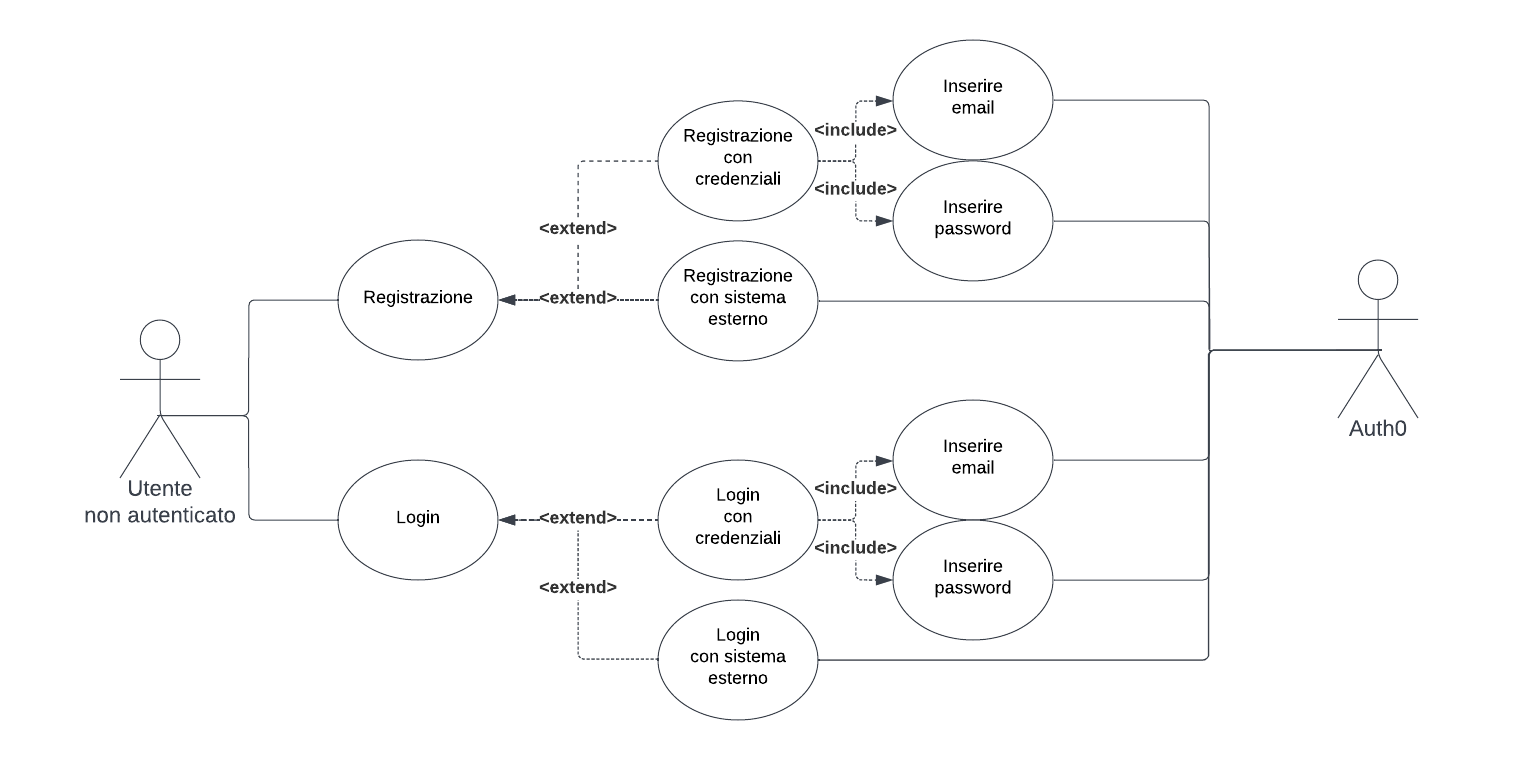
\includegraphics[width=0.7\textwidth]{img/Diagrammi/UseCases/AccessoRegistrazione.png}
    \end{center}

    \textbf{Diagramma:}
    \begin{center}
        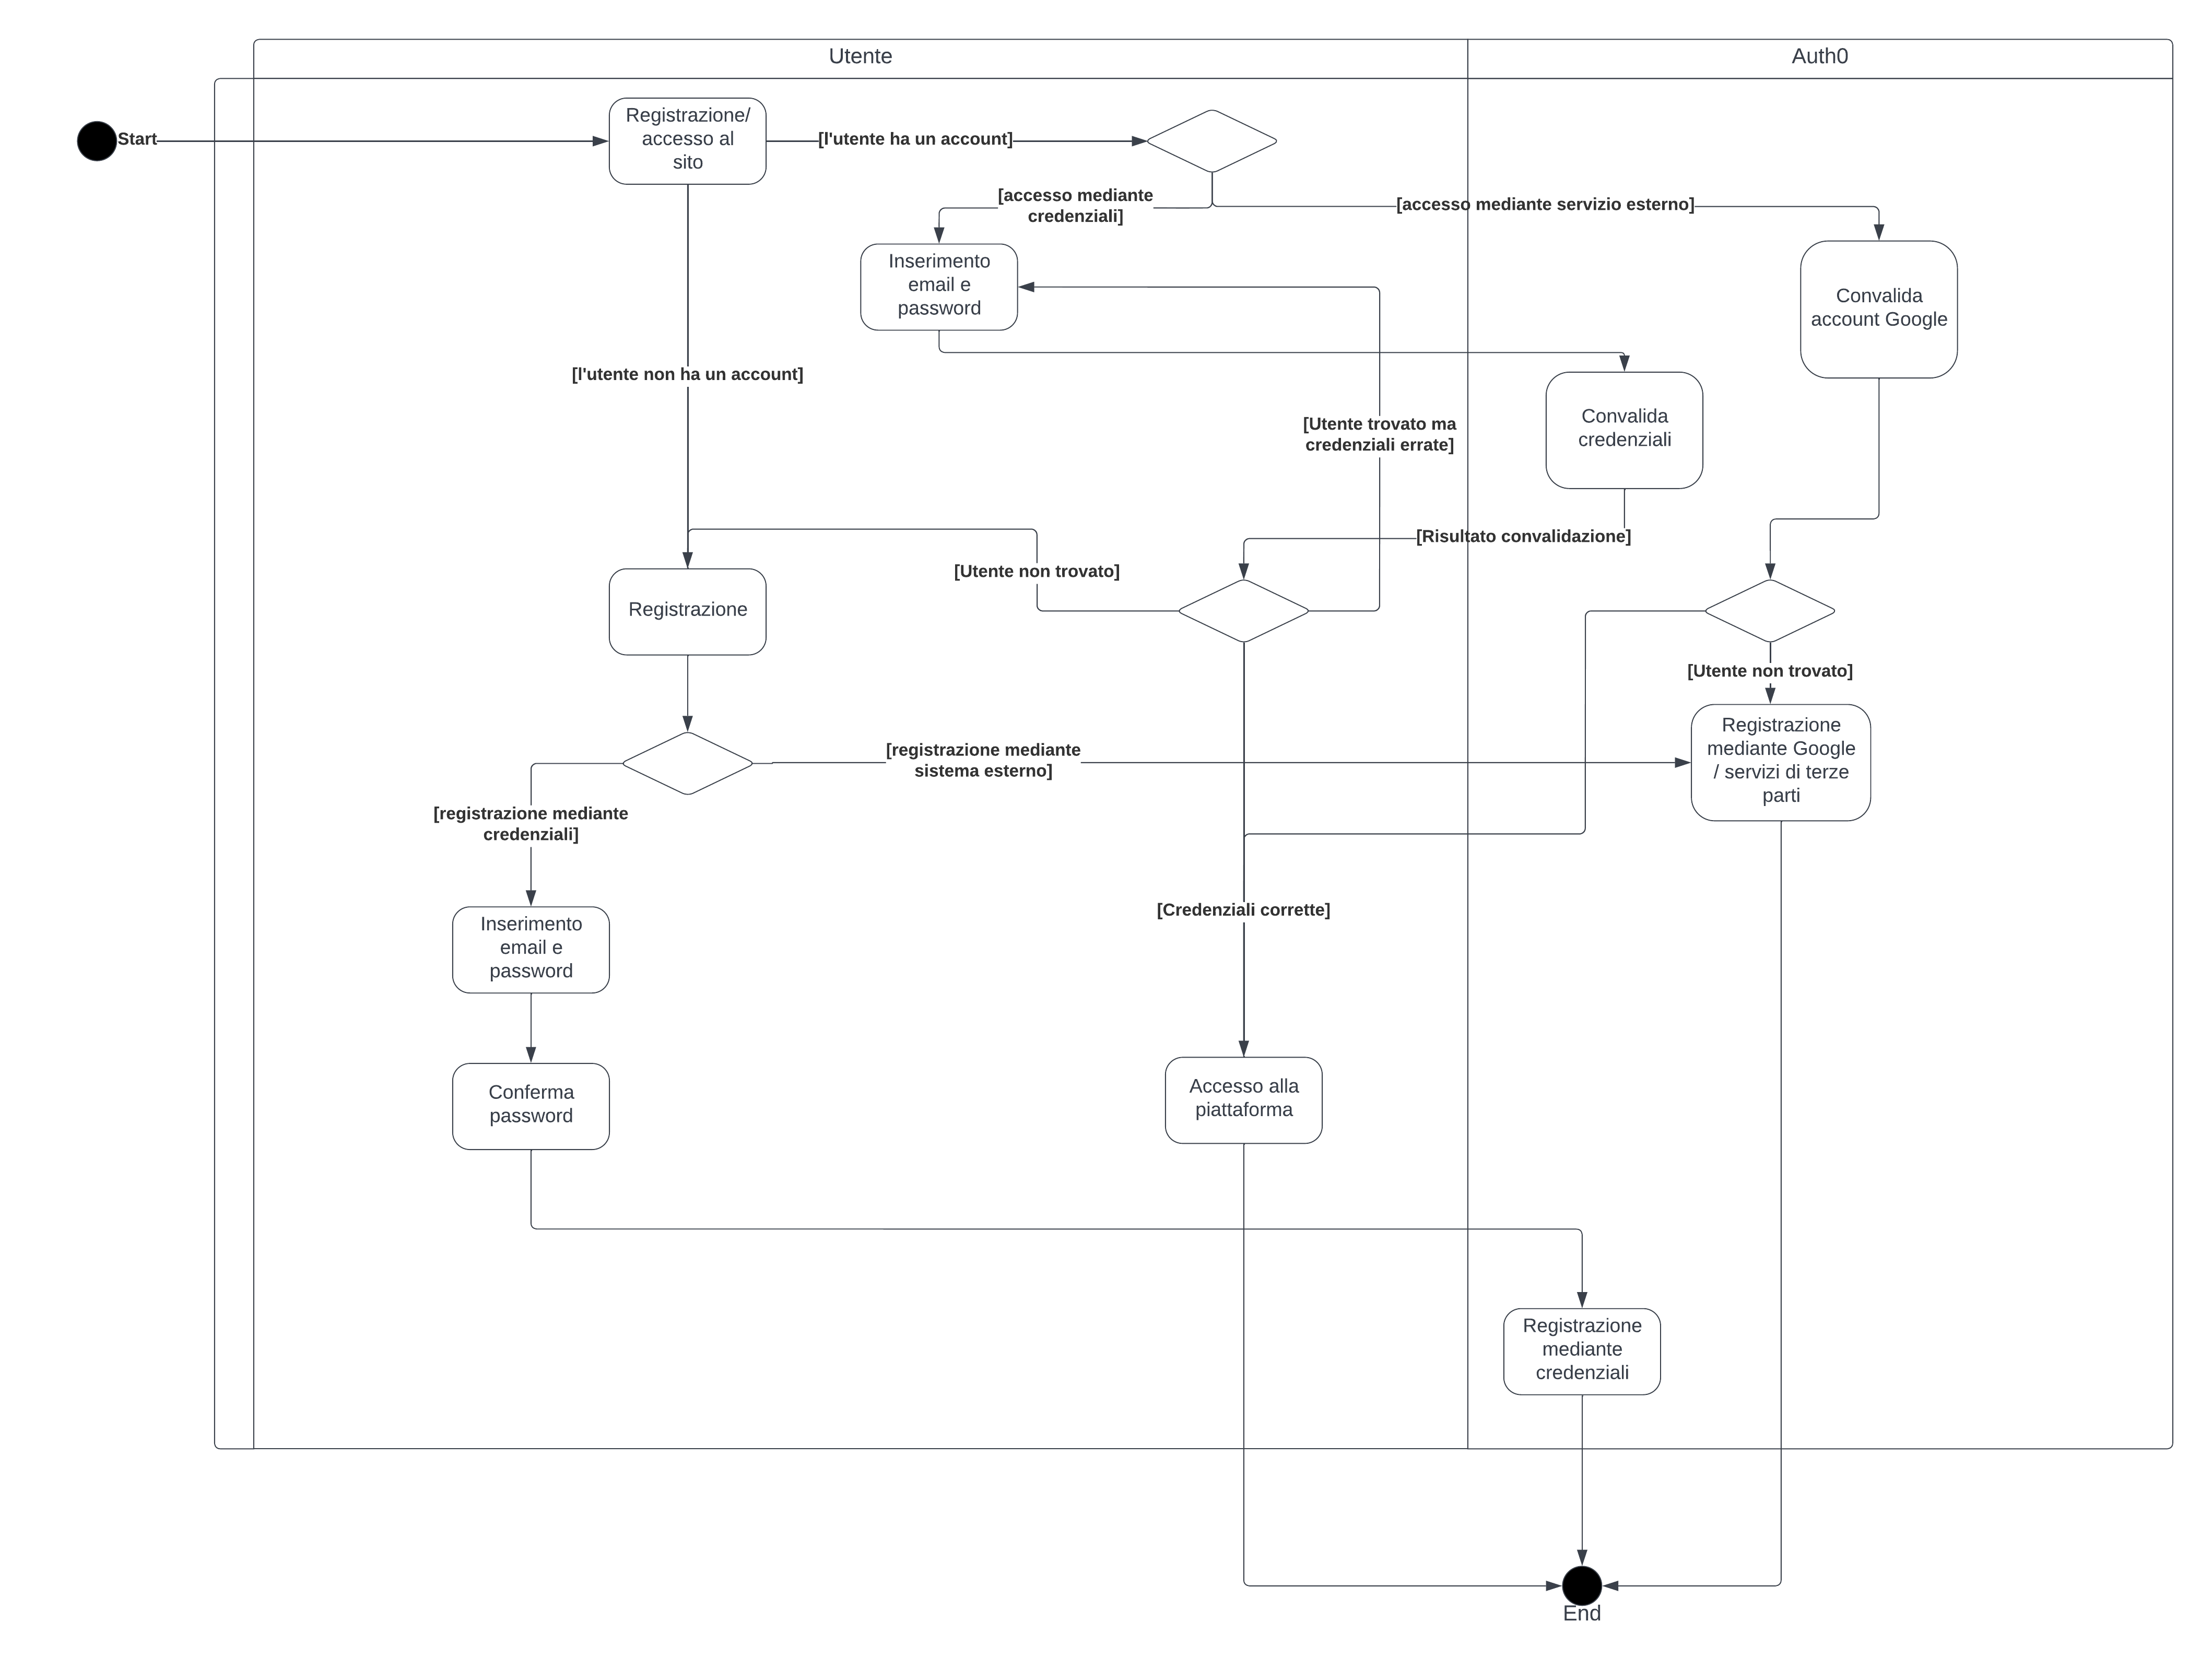
\includegraphics[width=0.7\textwidth]{img/Diagrammi/DS/DS_AccessoRegistrazione.png}
    \end{center}


    \newpage
    \elemento[Use case “Funzionalità di ciascuna tipologia di account”]{uc:TipiAccount}


    \begin{center}
        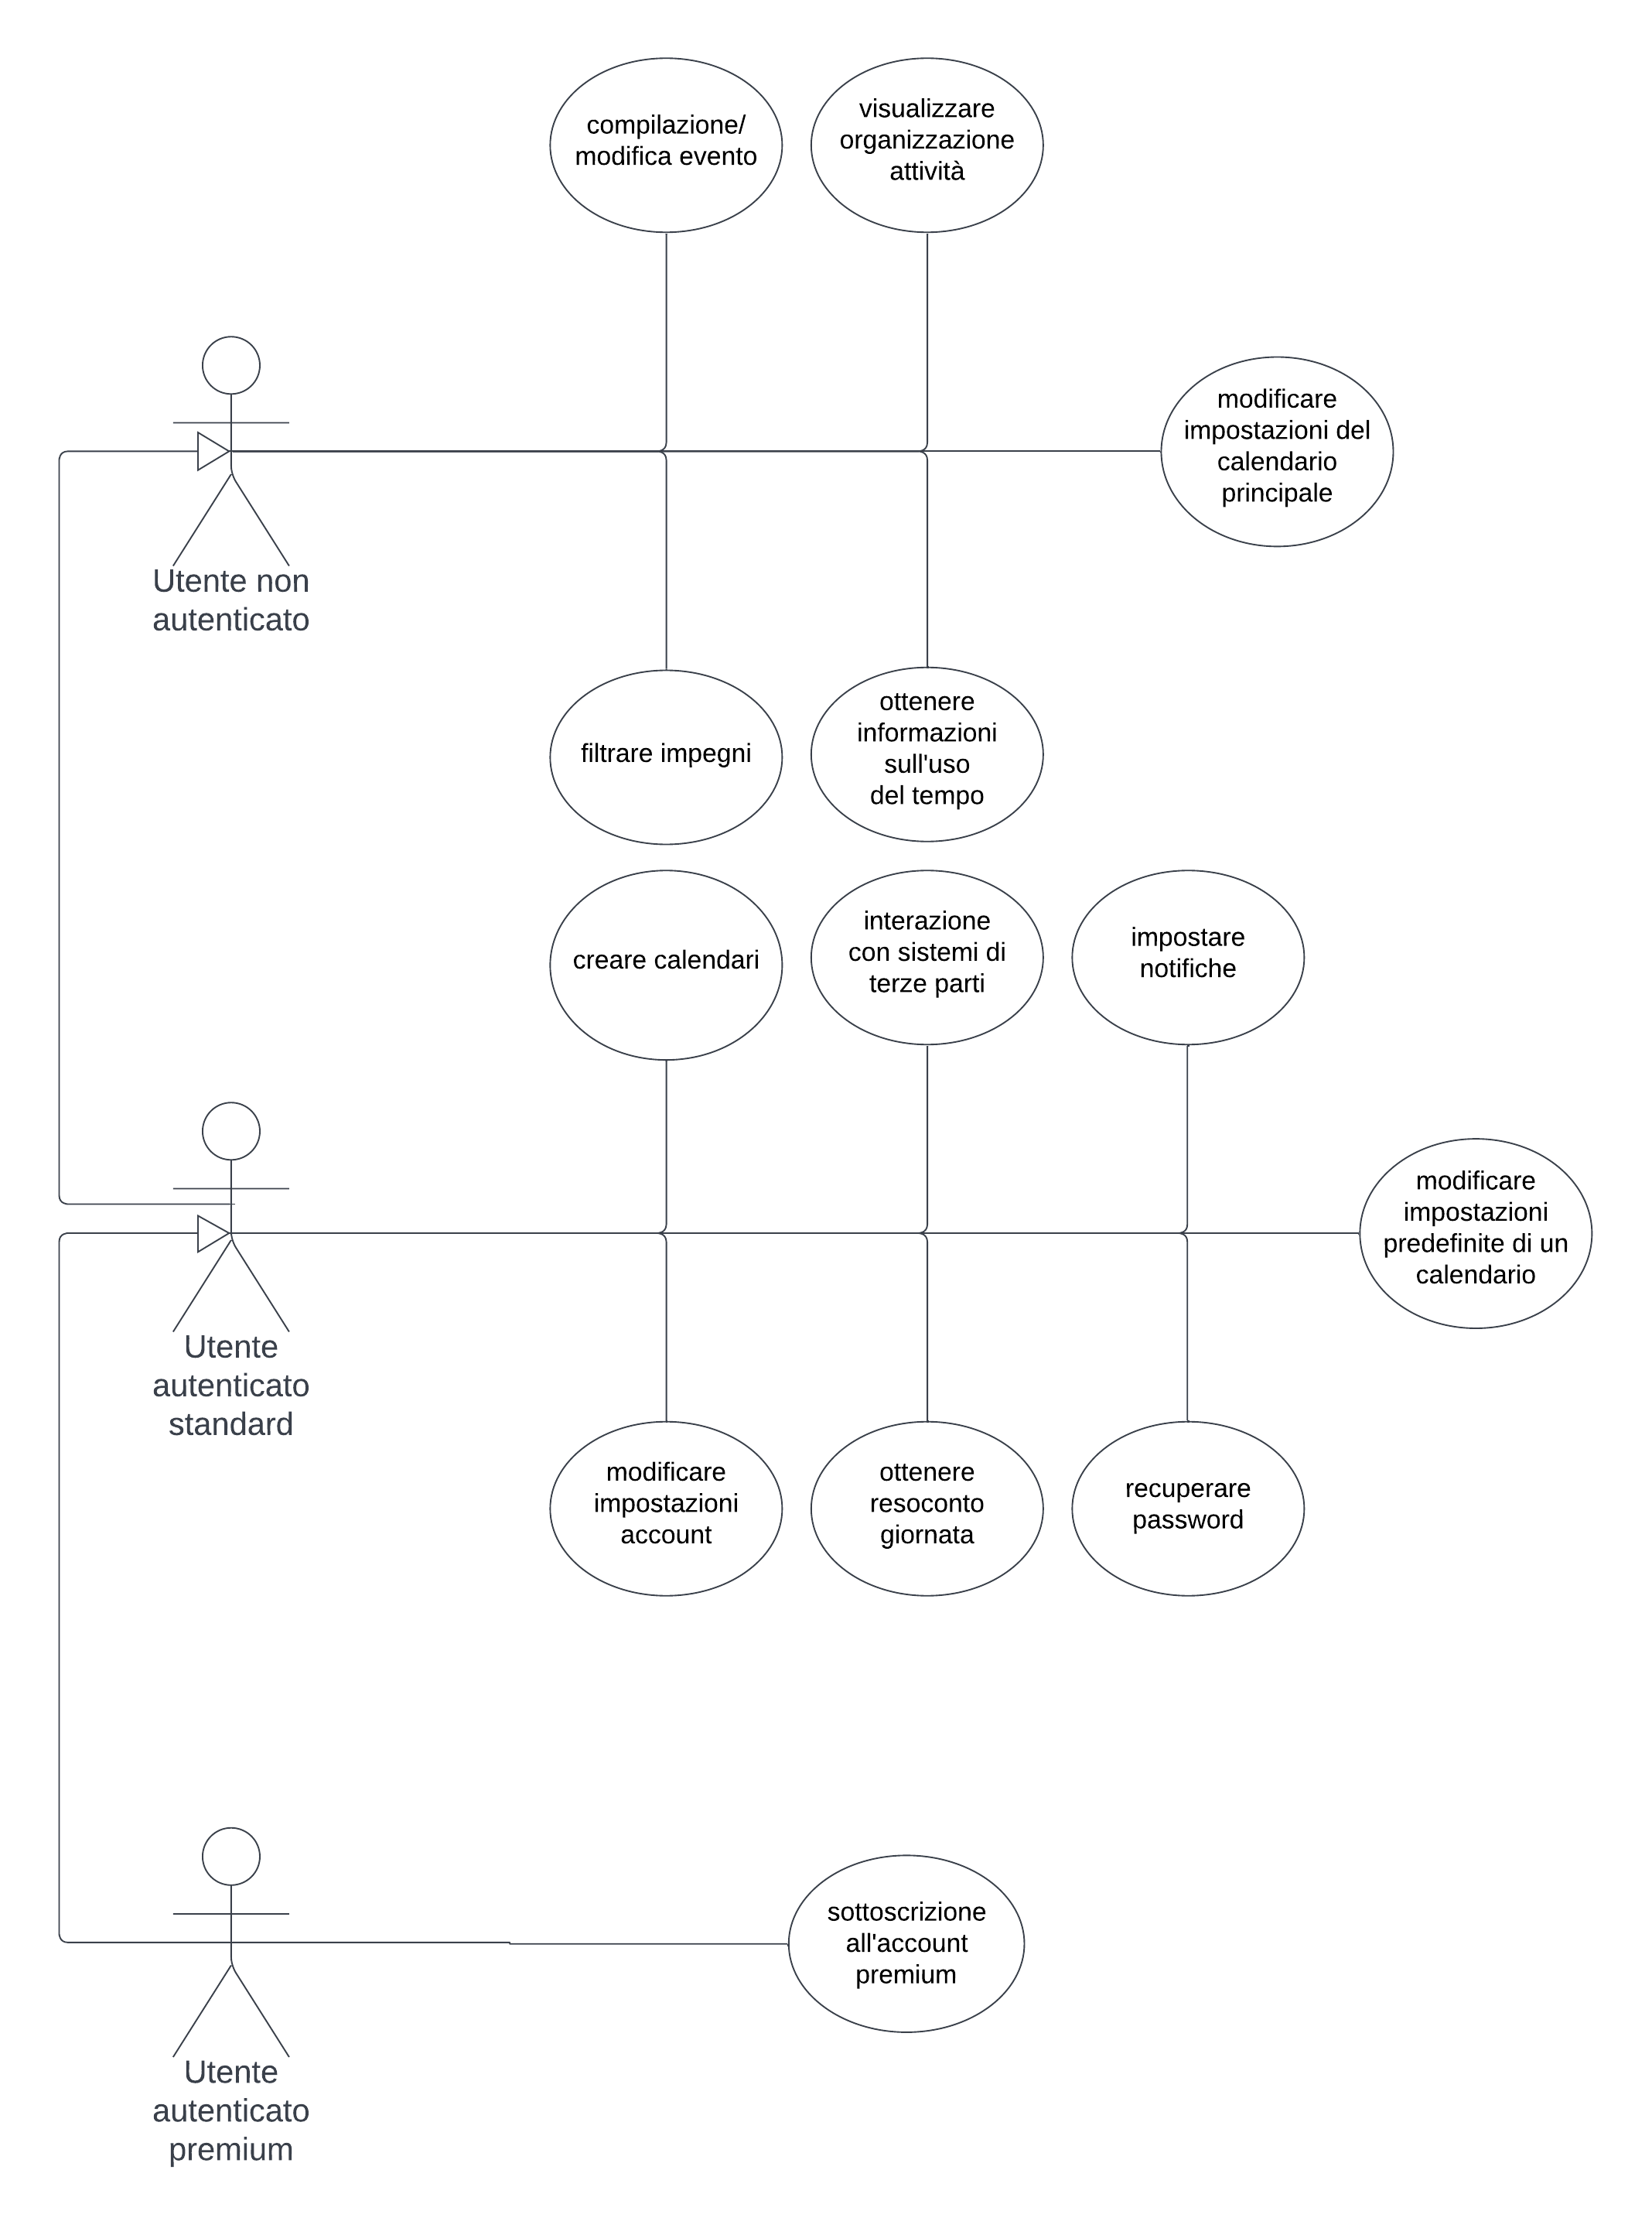
\includegraphics[width=0.4\textwidth]{img/Diagrammi/UseCases/FunzionalitaUtenti.png}
    \end{center}

    \textbf{Descrizione:}

    \textbf{Titolo:} funzionalità di ciascuna tipologia di account

    \textbf{Riassunto:} questo use case presenta in generale quali sono le funzionalità presenti per ciascuna tipologia di account. Tutte le funzionalità sotto presentate sono dettagliate nei successivi use case, che entreranno nello specifico di ciascuna funzionalità.

    \textbf{Descrizione:}
    \begin{enumerate}
        \item L'utente non autenticato, grazie alla modalità demo del sito, accede alle seguenti funzionalità:
              \begin{itemize}
                  \item compilazione/modifica evento;
                  \item visualizzare organizzazione attività;
                  \item modificare impostazioni del calendario principale;
                  \item ottenere informazioni sull'uso del tempo;
                  \item filtrare gli impegni.
              \end{itemize}
        \item L'utente autenticato standard accede alle seguenti funzionalità, da aggiungere a quelle dell'utente non autenticato:
              \begin{itemize}
                  \item creare calendari;
                  \item interazione con sistemi di terze parti;
                  \item impostare notifiche;
                  \item modificare impostazioni predefinite di un calendario;
                  \item recuperare password;
                  \item ottenere resoconto giornata;
                  \item modificare impostazioni account.
              \end{itemize}
        \item L'utente autenticato premium accede alle seguenti funzionalità, da aggiungere a quelle dell'utente autenticato standard:
              \begin{itemize}
                  \item sottoscrizione all'account premium, mediante un pagamento mensile.
              \end{itemize}
        \item Specifichiamo, quindi, che tutti gli use case validi per l'utente non autenticato, lo sono anche per quello autenticato standard e premium. Allo stesso modo gli use case per l'utente autenticato standard sono validi anche per l'utente autenticato premium.
    \end{enumerate}






    \newpage
    \elemento[Use case “Sottoscrizione all'account premium”]{uc:SottoscrizioneAccountPremium}


    \begin{center}
        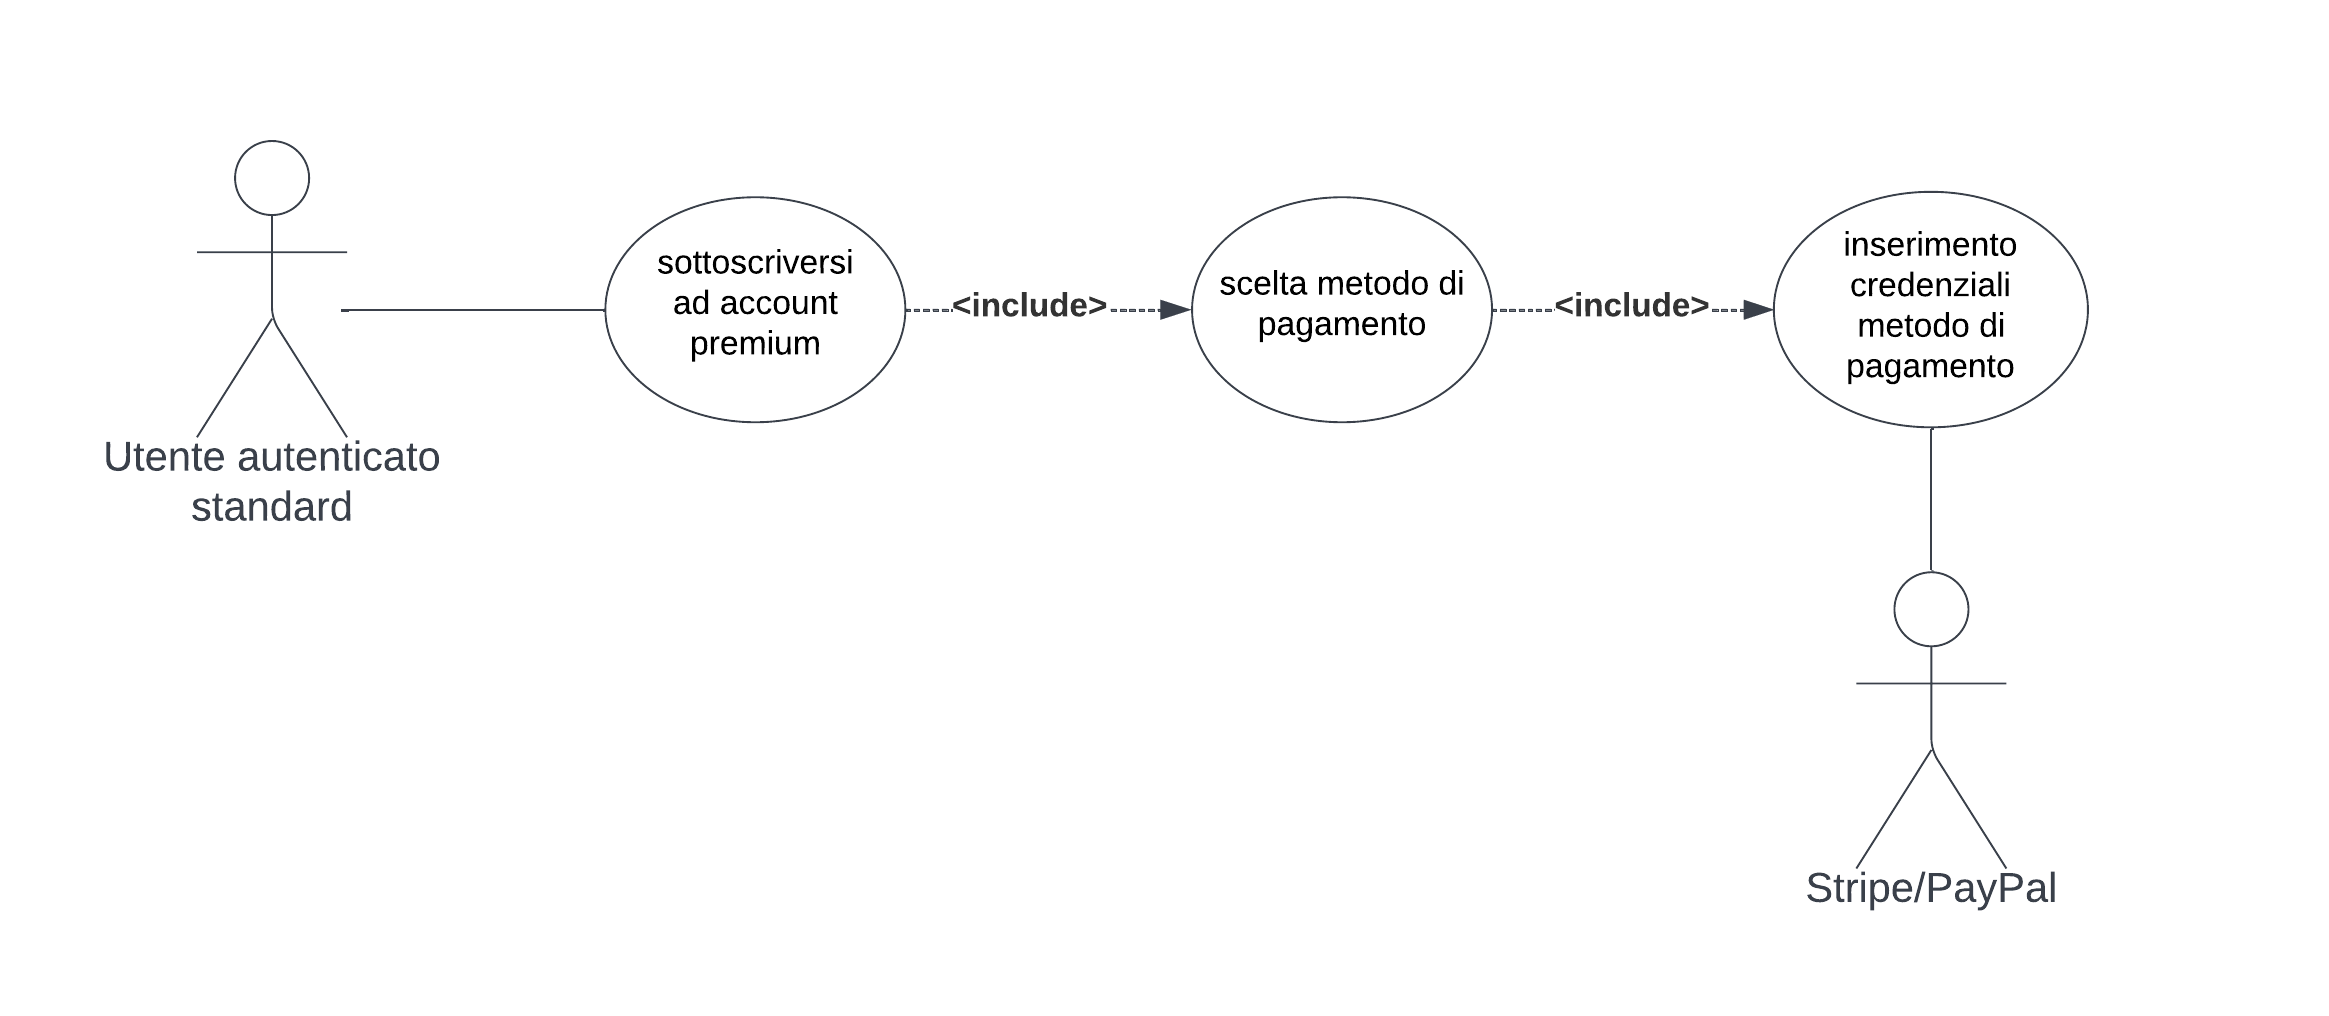
\includegraphics[width=0.7\textwidth]{img/Diagrammi/UseCases/UtentePremium.png}
    \end{center}

    \textbf{Descrizione:}

    \textbf{Titolo:} sottoscrizione all'account premium.

    \textbf{Riassunto:} questo use case descrive come avviene la sottoscrizione all'account premium mediante un abbonamento a pagamento.

    \textbf{Descrizione:}
    \begin{enumerate}
        \item L'utente autenticato standard, nella sezione “impostazioni account”, preme il tasto il campo: “Abbonarsi”.
        \item Una volta selezionato questo campo, l'utente autenticato standard dovrà scegliere tra 2 possibili metodi di pagamento predefiniti: Stripe o PayPal.
        \item Dopo aver scelto uno dei metodi di pagamento, l'utente autenticato standard verrà indirizzato nella pagina del metodo di pagamento selezionato, dove dovrà inserire le proprie credenziali riguardanti il suo account del sistema esterno di pagamento. \ref{uc:ExceptionCredenzialiSistemaDiPagamento}
        \item Una volta che l'utente autenticato standard inserirà queste credenziali, l'utente autenticato standard avrà aggiunto correttamente al suo account il metodo di pagamento dell'abbonamento.
        \item L'abbonamento all'account premium, a questo punto, partirà automaticamente con un costo mensile di 15 euro. Ogni mese il pagamento verrà fatto in maniera automatica mediante il metodo di pagamento inserito, che può essere modificato in “Impostazioni Account”. L'account premium può essere disabilitato, in ogni momento, da “Impostazioni Account” premendo sul tasto “Disattiva”, che appare al posto del tasto “Abbonarsi” solo nel caso in cui si ha l'abbonamento all'account premium.
    \end{enumerate}

    %\todo{Forse dovremmo fare un requisito funzionale per disabilitare account premium?!}

    \textbf{Exceptions:}
    \begin{enumerate}[label=\textbf{[exception \arabic{enumii}]}, ref= \textbf{[exception \arabic{enumii}]}]
        \elemento{uc:ExceptionCredenzialiSistemaDiPagamento} L'inserimento delle credenziali andrà avanti finché l'utente non inserirà delle credenziali corrette del sistema esterno del metodo di pagamento scelto. Infatti l'utente autenticato standard va avanti con la procedura della sottoscrizione solo una volta che ha inserito delle credenziali corrette.
    \end{enumerate}
    %\todo{Qua c'è un problema non possiamo mettere la sottoscrizione dalle impostazioni Account sennò dopo dobbiamo andare a modificare in realtà impostazioni account e il suo state diagram}






    \newpage
    \elemento[Use case “Gestione di calendari”]{uc:GestioneCalendari}


    \begin{center}
        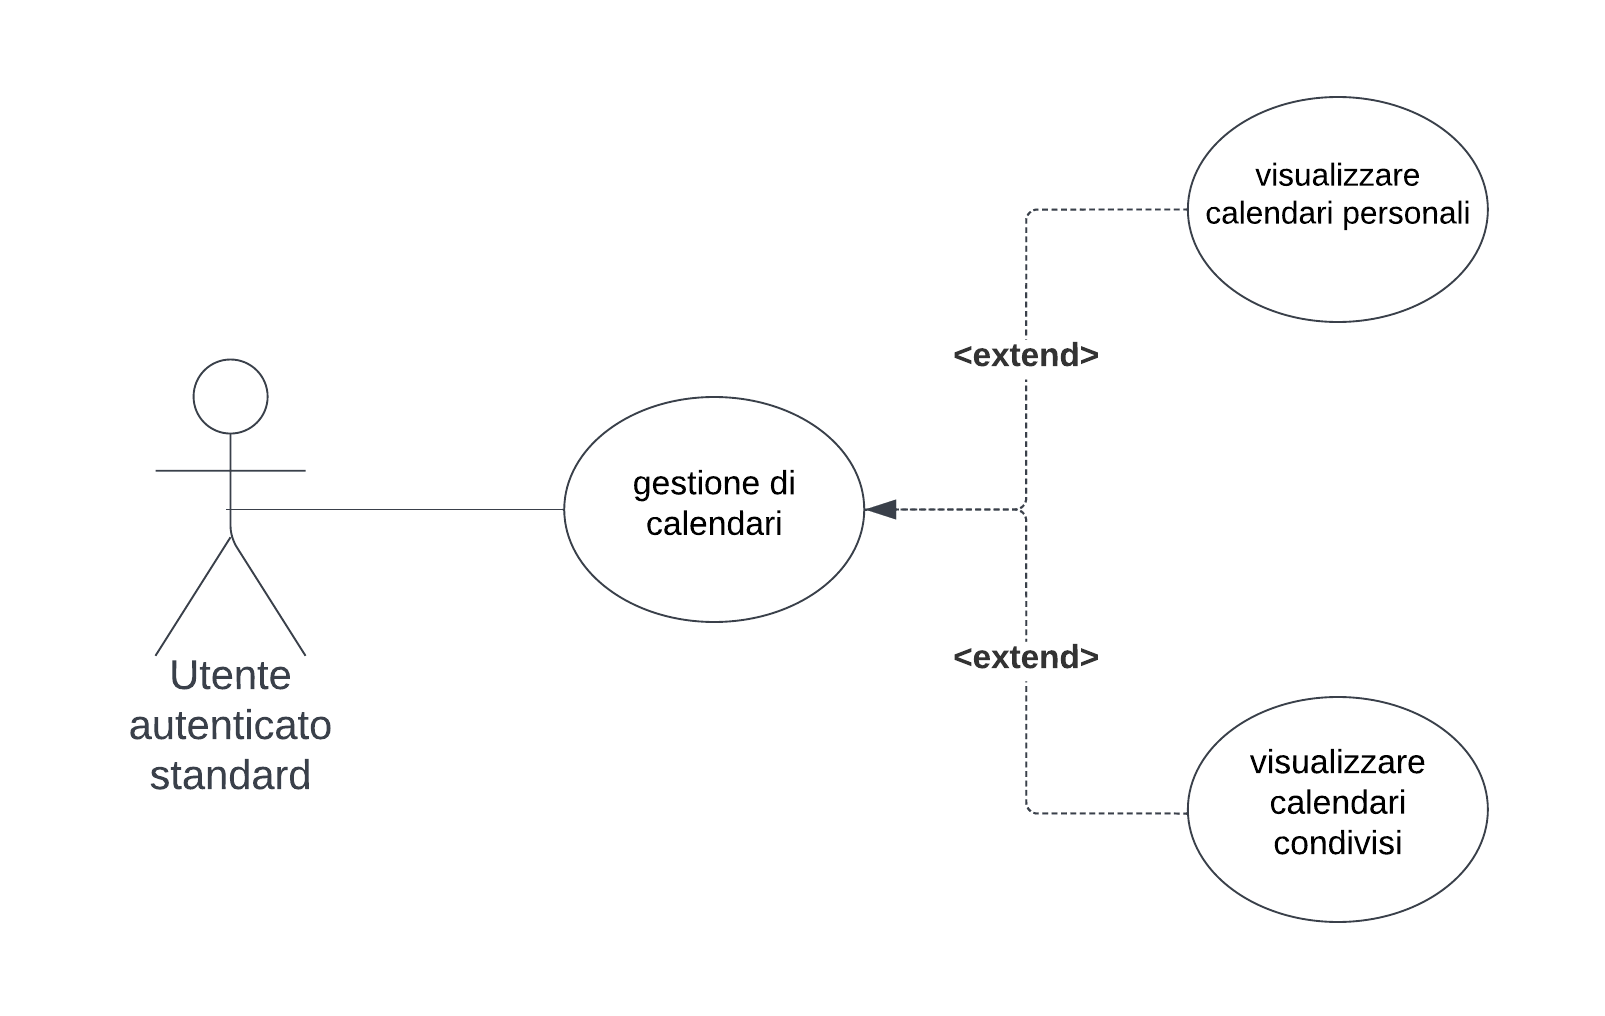
\includegraphics[width=0.7\textwidth]{img/Diagrammi/UseCases/CondivisioneCalendario.png}
    \end{center}

    \textbf{Descrizione:}

    \textbf{Titolo:} gestione di calendari

    \textbf{Riassunto:} questo use descrive come l'utente autenticato standard può visualizzare e gestire i calendari personali e quelli condivisi.

    \textbf{Descrizione:}
    \begin{enumerate}
        \item Dalla sezione Calendari, l'utente può visualizzare i suoi calendari personali e i calendari condivisi con altre persone.
        \item L'utente autenticato standard, da questa sezione, può selezionare quali calendari far apparire nella schermata “Calendario” in modo tale da osservare quali siano gli eventi presenti in un calendario specifico.
        \item Aprendo la sottosezione del calendario “Principale”, l'utente visualizza tutti i suoi calendari personali riguardo alle varie attività da svolgere. Il numero di calendari personali dipende dal tipo di account dell'utente autenticato: l'utente autenticato standard può avere al massimo 5 calendari personali, invece l'utente autenticato premium può avere un numero illimitato di calendari personali.
        \item Sotto il calendario “Principale”, sono presenti tutti i calendari condivisi (\ref{uc:ExtensionVisualizzazioneCalendariCondivisi}). Il numero di calendari condivisi che può avere un utente autenticato dipende dalla tipologia di account: l'utente autenticato standard può avere al massimo 3 calendari condivisi, invece l'utente autenticato premium può avere un numero illimitato di calendari personali.
    \end{enumerate}


    \textbf{Extension:}
    \begin{enumerate}[label=\textbf{[extension \arabic{enumii}]}, ref= \textbf{[extension \arabic{enumii}]}]
        \elemento{uc:ExtensionVisualizzazioneCalendariCondivisi} L'utente autenticato standard può visualizzare quali siano i calendari condivisi anche osservando una piccola immagine stilizzata di persone alla destra del nome dei calendari condivisi.
    \end{enumerate}






    \newpage
    \elemento[Use case “Creazione/modifica evento”]{uc:CreazioneModificaEvento}

    \begin{center}
        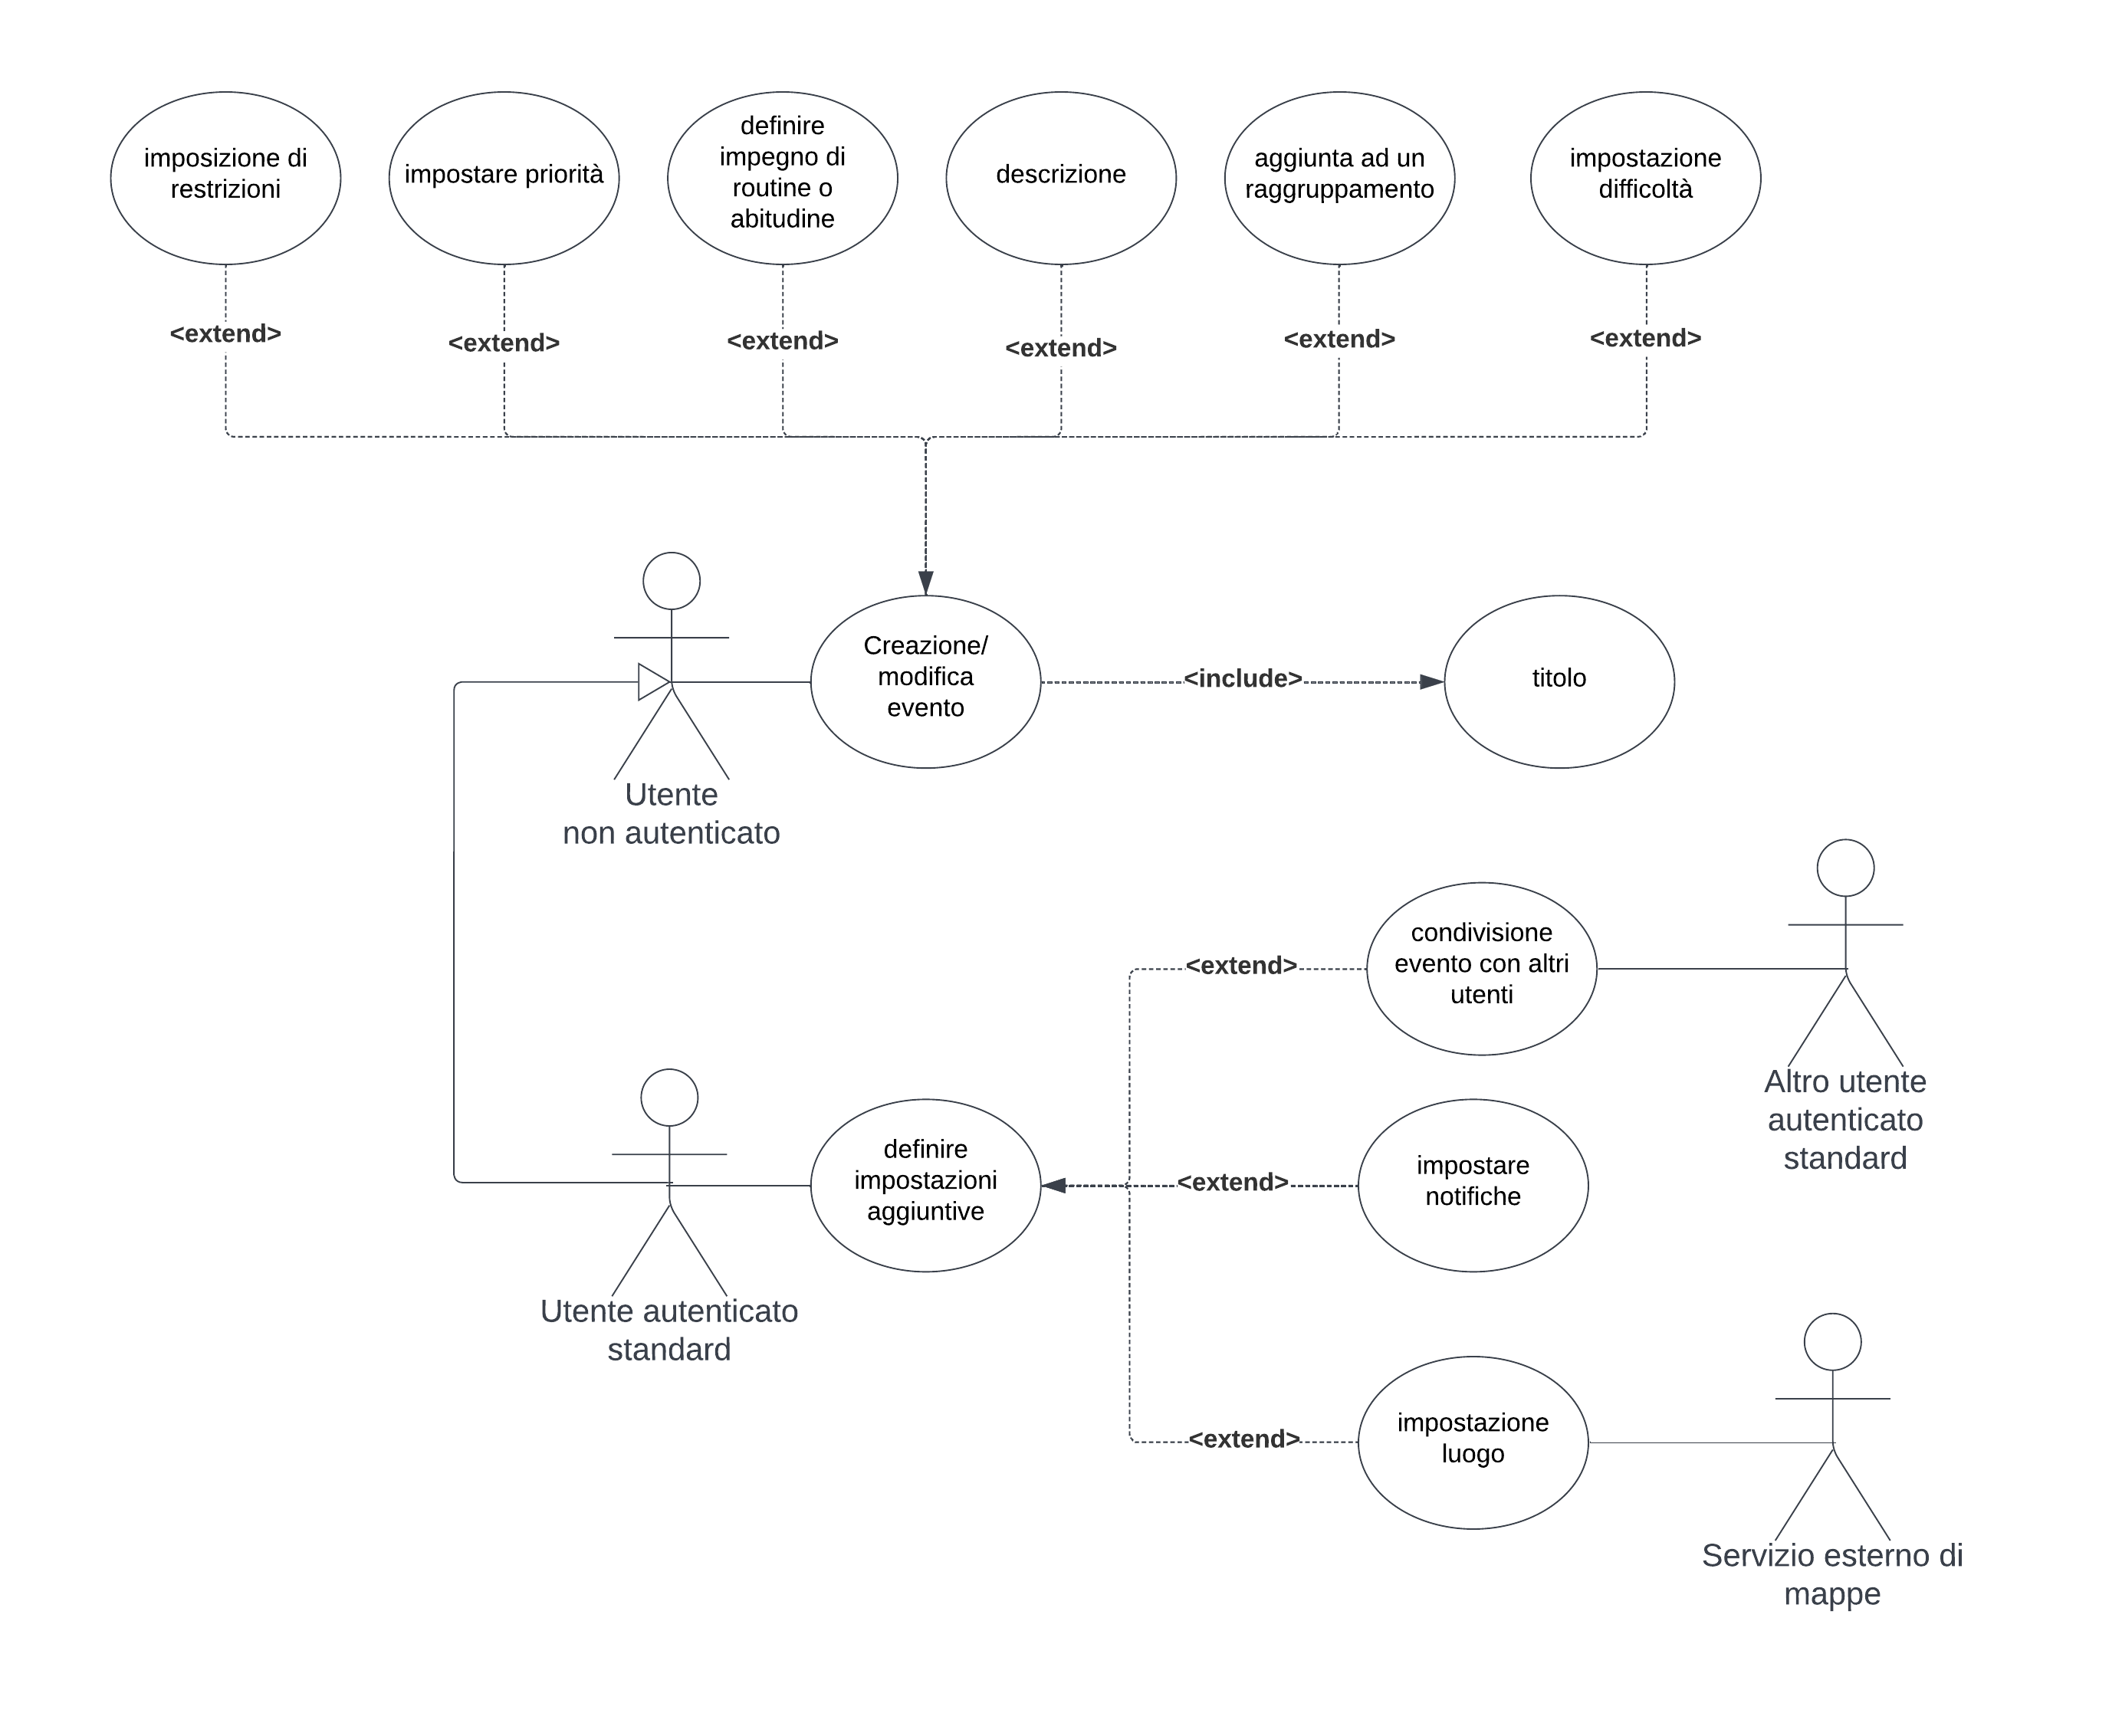
\includegraphics[width=0.7\textwidth]{img/Diagrammi/UseCases/CreazioneModificaEvento.png}
    \end{center}


    \textbf{Diagramma:}
    \begin{center}
        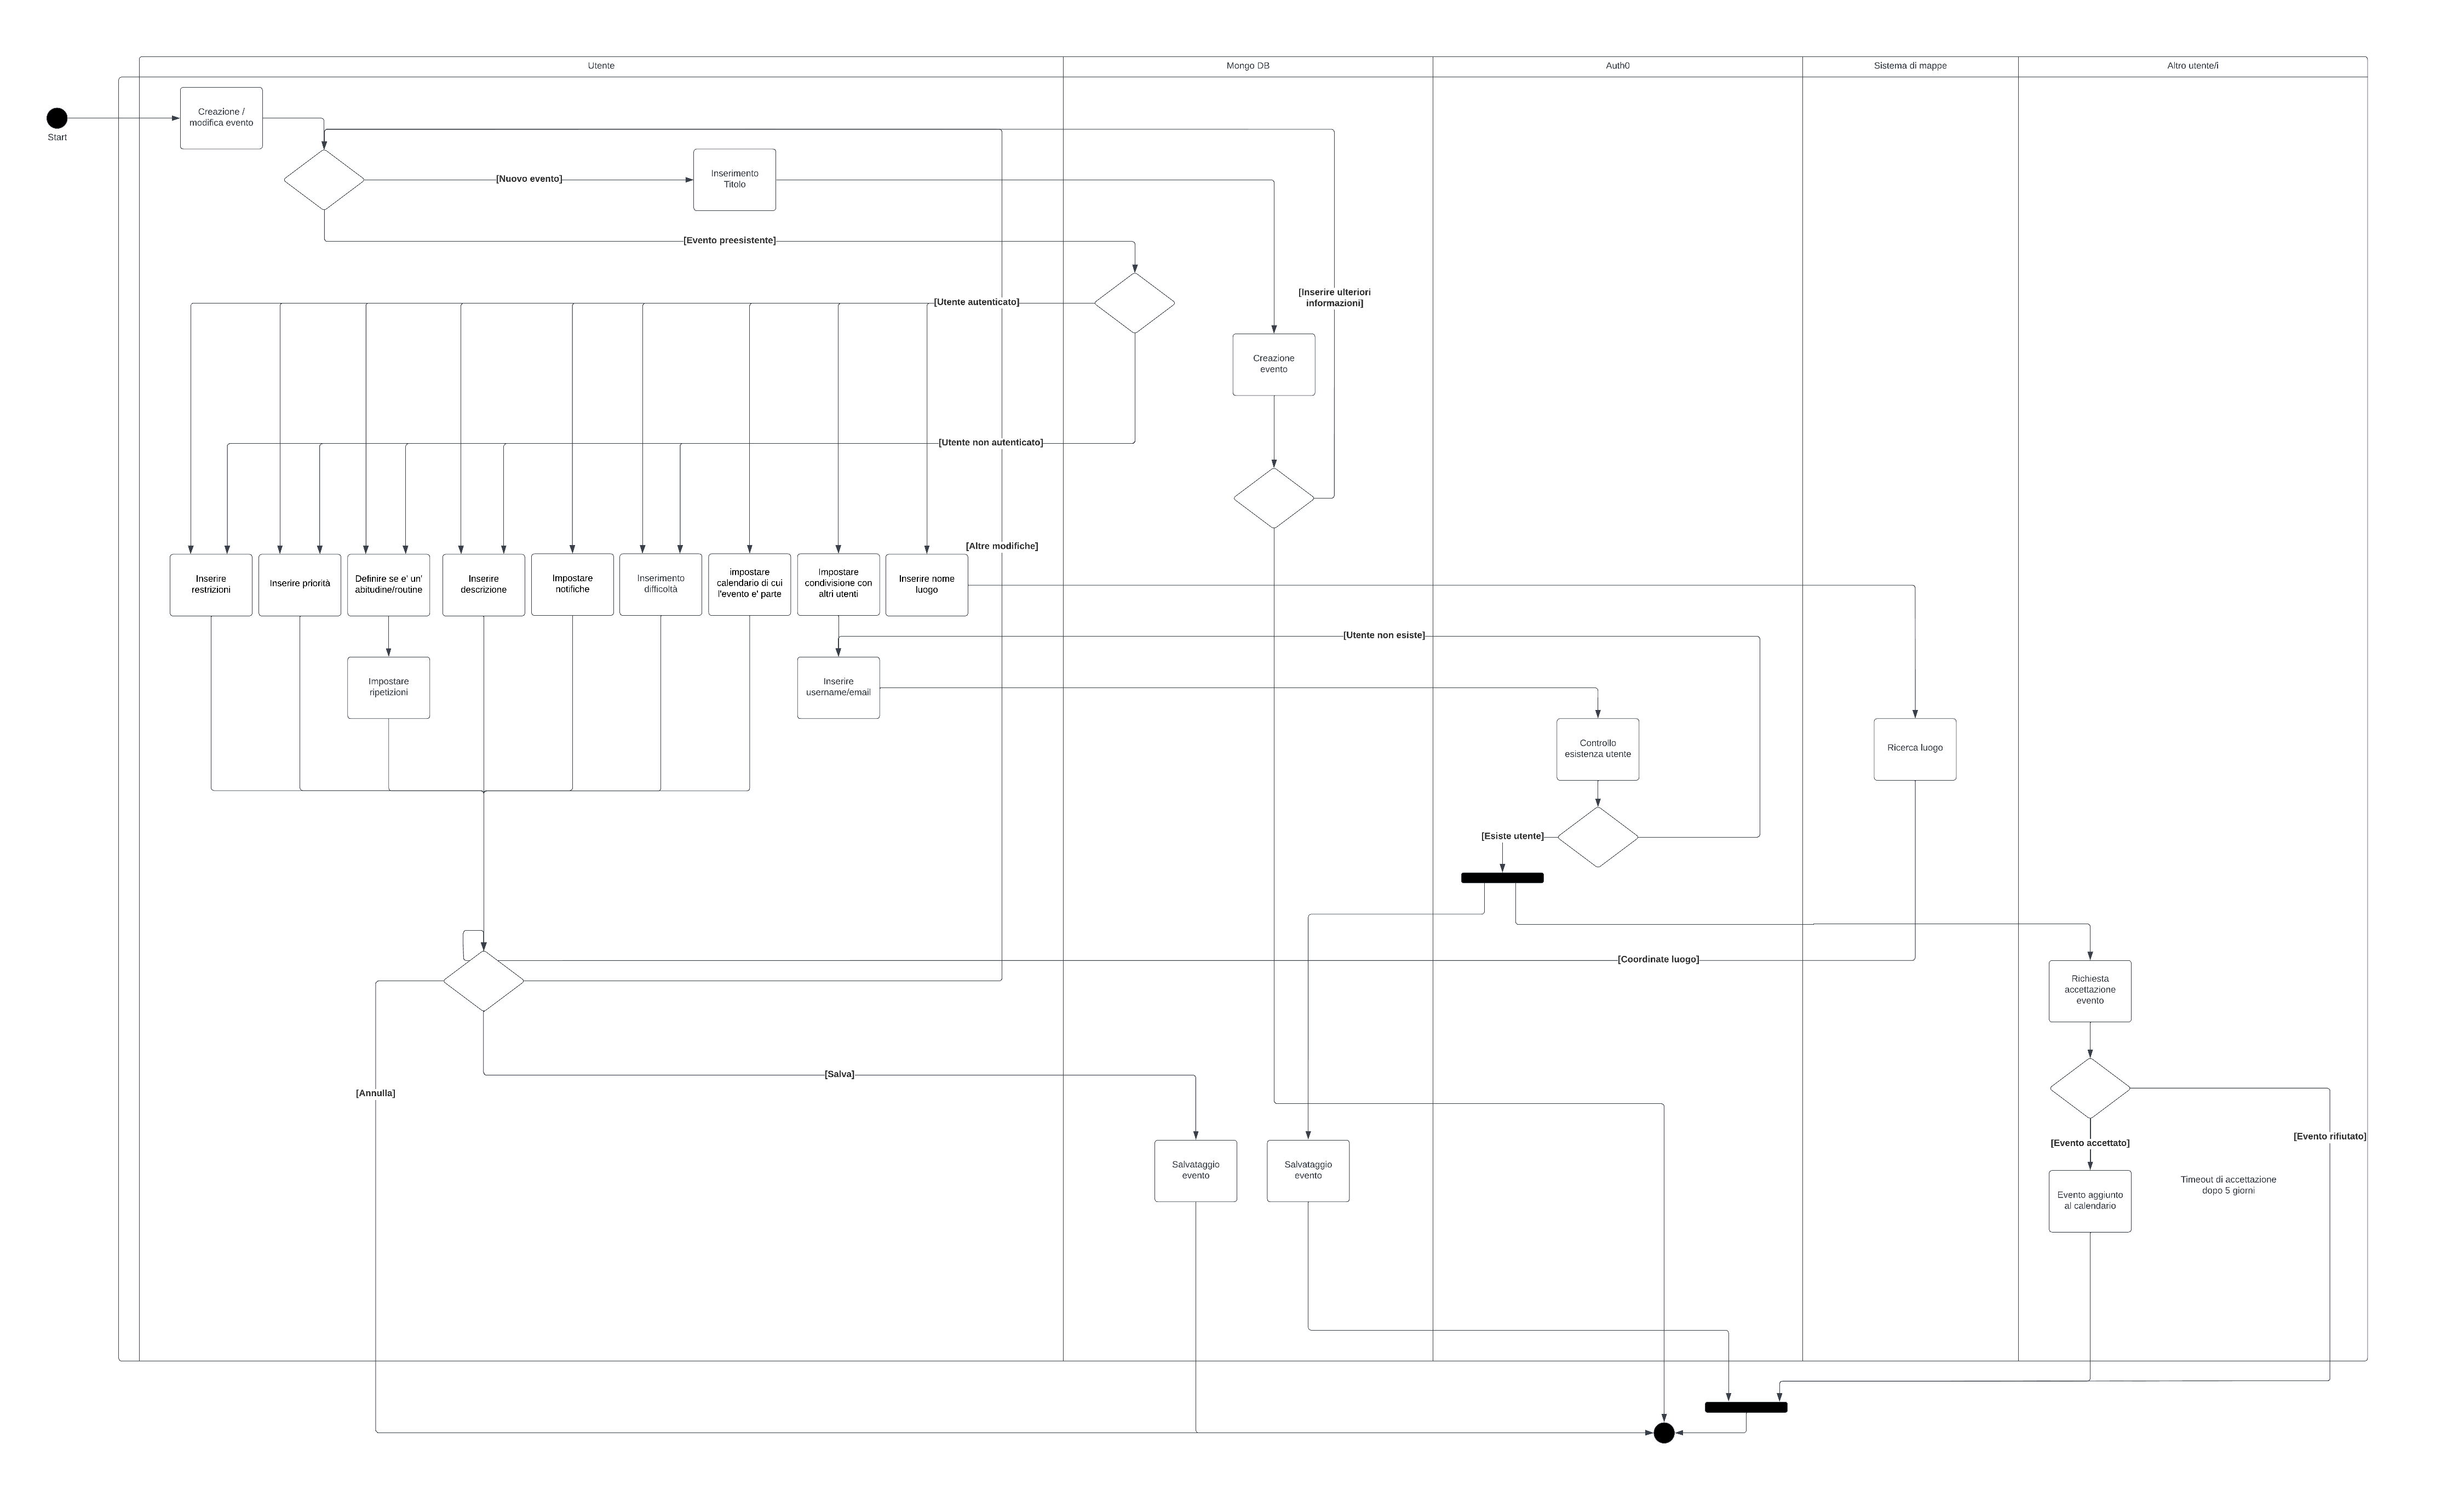
\includegraphics[width=0.7\textwidth]{img/Diagrammi/DS/DS_CreazioneModificaEvento.png}
    \end{center}




    \newpage
    \elemento[Use case “Visualizza attività nel calendario”]{uc:VisualizzazioneEventiCalendario}


    \begin{center}
        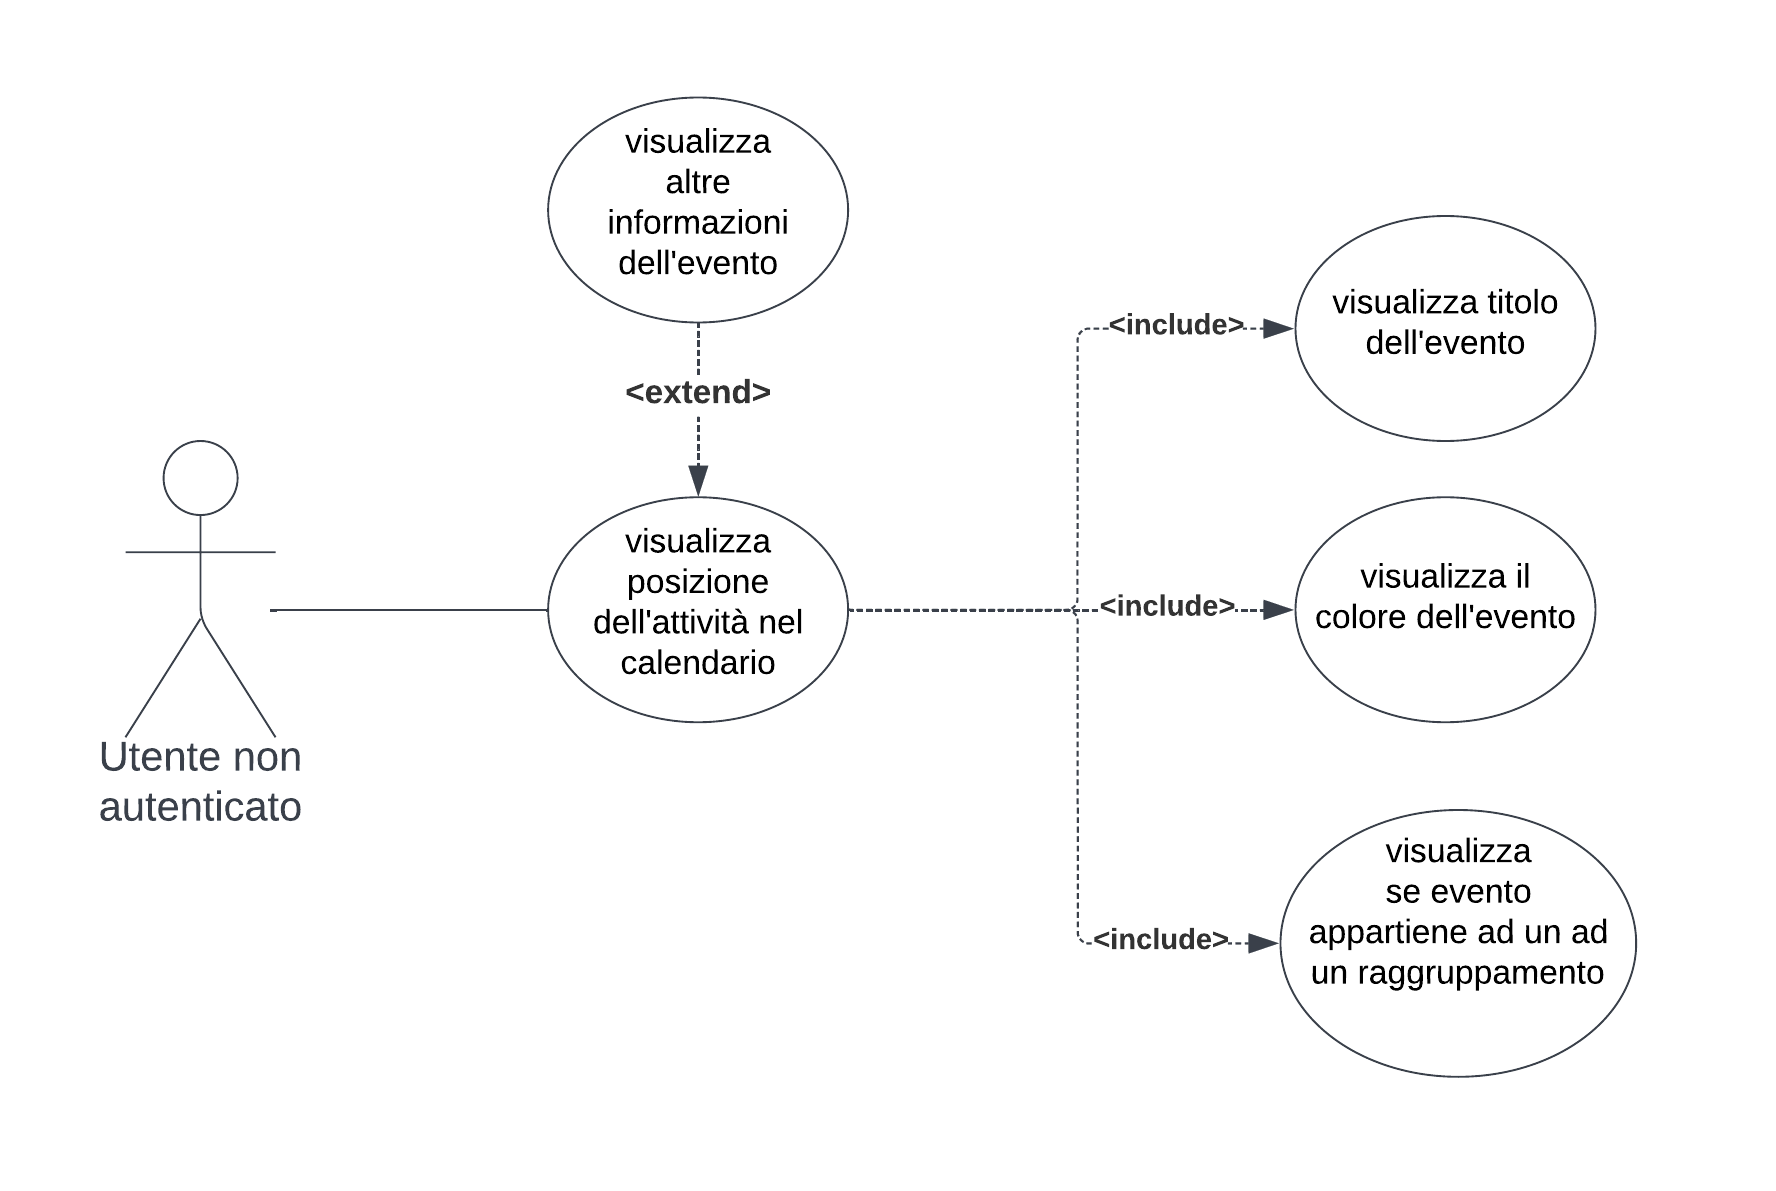
\includegraphics[width=0.7\textwidth]{img/Diagrammi/UseCases/InserimentoAutomaticoCalendario.png}
    \end{center}

    \textbf{Descrizione:}

    \textbf{Titolo:} Organizzazione attività

    \textbf{Riassunto:} questo use case descrive come l'utente non autenticato visualizza l'evento nel proprio calendario e quali informazioni può ottenere dal blocco dell'evento presente nella schermata “Calendario”.

    \textbf{Descrizioni:}
    \begin{enumerate}
        \item Dopo la compilazione dell'evento da aggiungere, l'utente non autenticato visualizza tale evento in un blocco nella schermata Calendario.
        \item Nel caso in cui l'utente non autenticato, in fase di compilazione dell'evento da aggiungere, non avesse definito data, ora e durata di tale attività, il sistema inserisce autonomamente e automaticamente l'impegno nel calendario secondo i seguenti criteri, i quali l'utente non autenticato può aver definito nella compilazione dell'evento: %\todo{[exception 1] In nche senso, a cosa fa riferimento?}
              \begin{itemize}
                  \item difficoltà dell' evento, ovvero quanto è complesso l'evento per completarlo;
                  \item priorità;
                  \item durata;
              \end{itemize}
        \item Dal blocco dell'evento nel calendario, l'utente non autenticato può visualizzare immediatamente alcune informazioni riguardo l'evento:
              \begin{itemize}
                  \item titolo;
                  \item colore dell'evento: da questa informazione l'utente non autenticato può comprendere a quale calendario o raggruppamento appartiene l'evento; infatti il colore dell'evento %\todo{corrisponde al colore del calendario al raggruppamento a cui appartiene (ricordiamo che nel caso di utente non autenticato l'unico colore presente sarà quello del calendario “principale”, in quanto non avrà possibilità di creare altri calendari”).}
                  \item se appartiene l'evento appartiene ad un raggruppamento, visualizza una denominazione sopra il titolo dell'evento che indica il raggruppamento, che è un insieme di attività del calendario principale.
              \end{itemize}
        \item L'utente non autenticato premendo sull'evento fa apparire un pop-up dove può visualizzare tutte le informazioni di tale evento, ovvero tutte quelle sopra descritte e:
              \begin{itemize}
                  \item descrizione dell'evento;
                  \item se l'evento è un'abitudine;
                  \item difficoltà dell'evento;
              \end{itemize}
        \item Nel caso di un utente autenticato standard, nel pop-up di visualizzazione di informazioni aggiuntive riguardo un evento saranno presenti altri campi, ovvero:
              \begin{itemize}
                  \item luogo dove si terrà l'evento;
                  \item utenti a cui è condiviso l'evento;
                  \item quando è impostata la notifica dell'evento.
              \end{itemize}
    \end{enumerate}





    \newpage
    \elemento[Use case “Resoconto giornata”]{uc:ResocontoGiornata}


    \begin{center}
        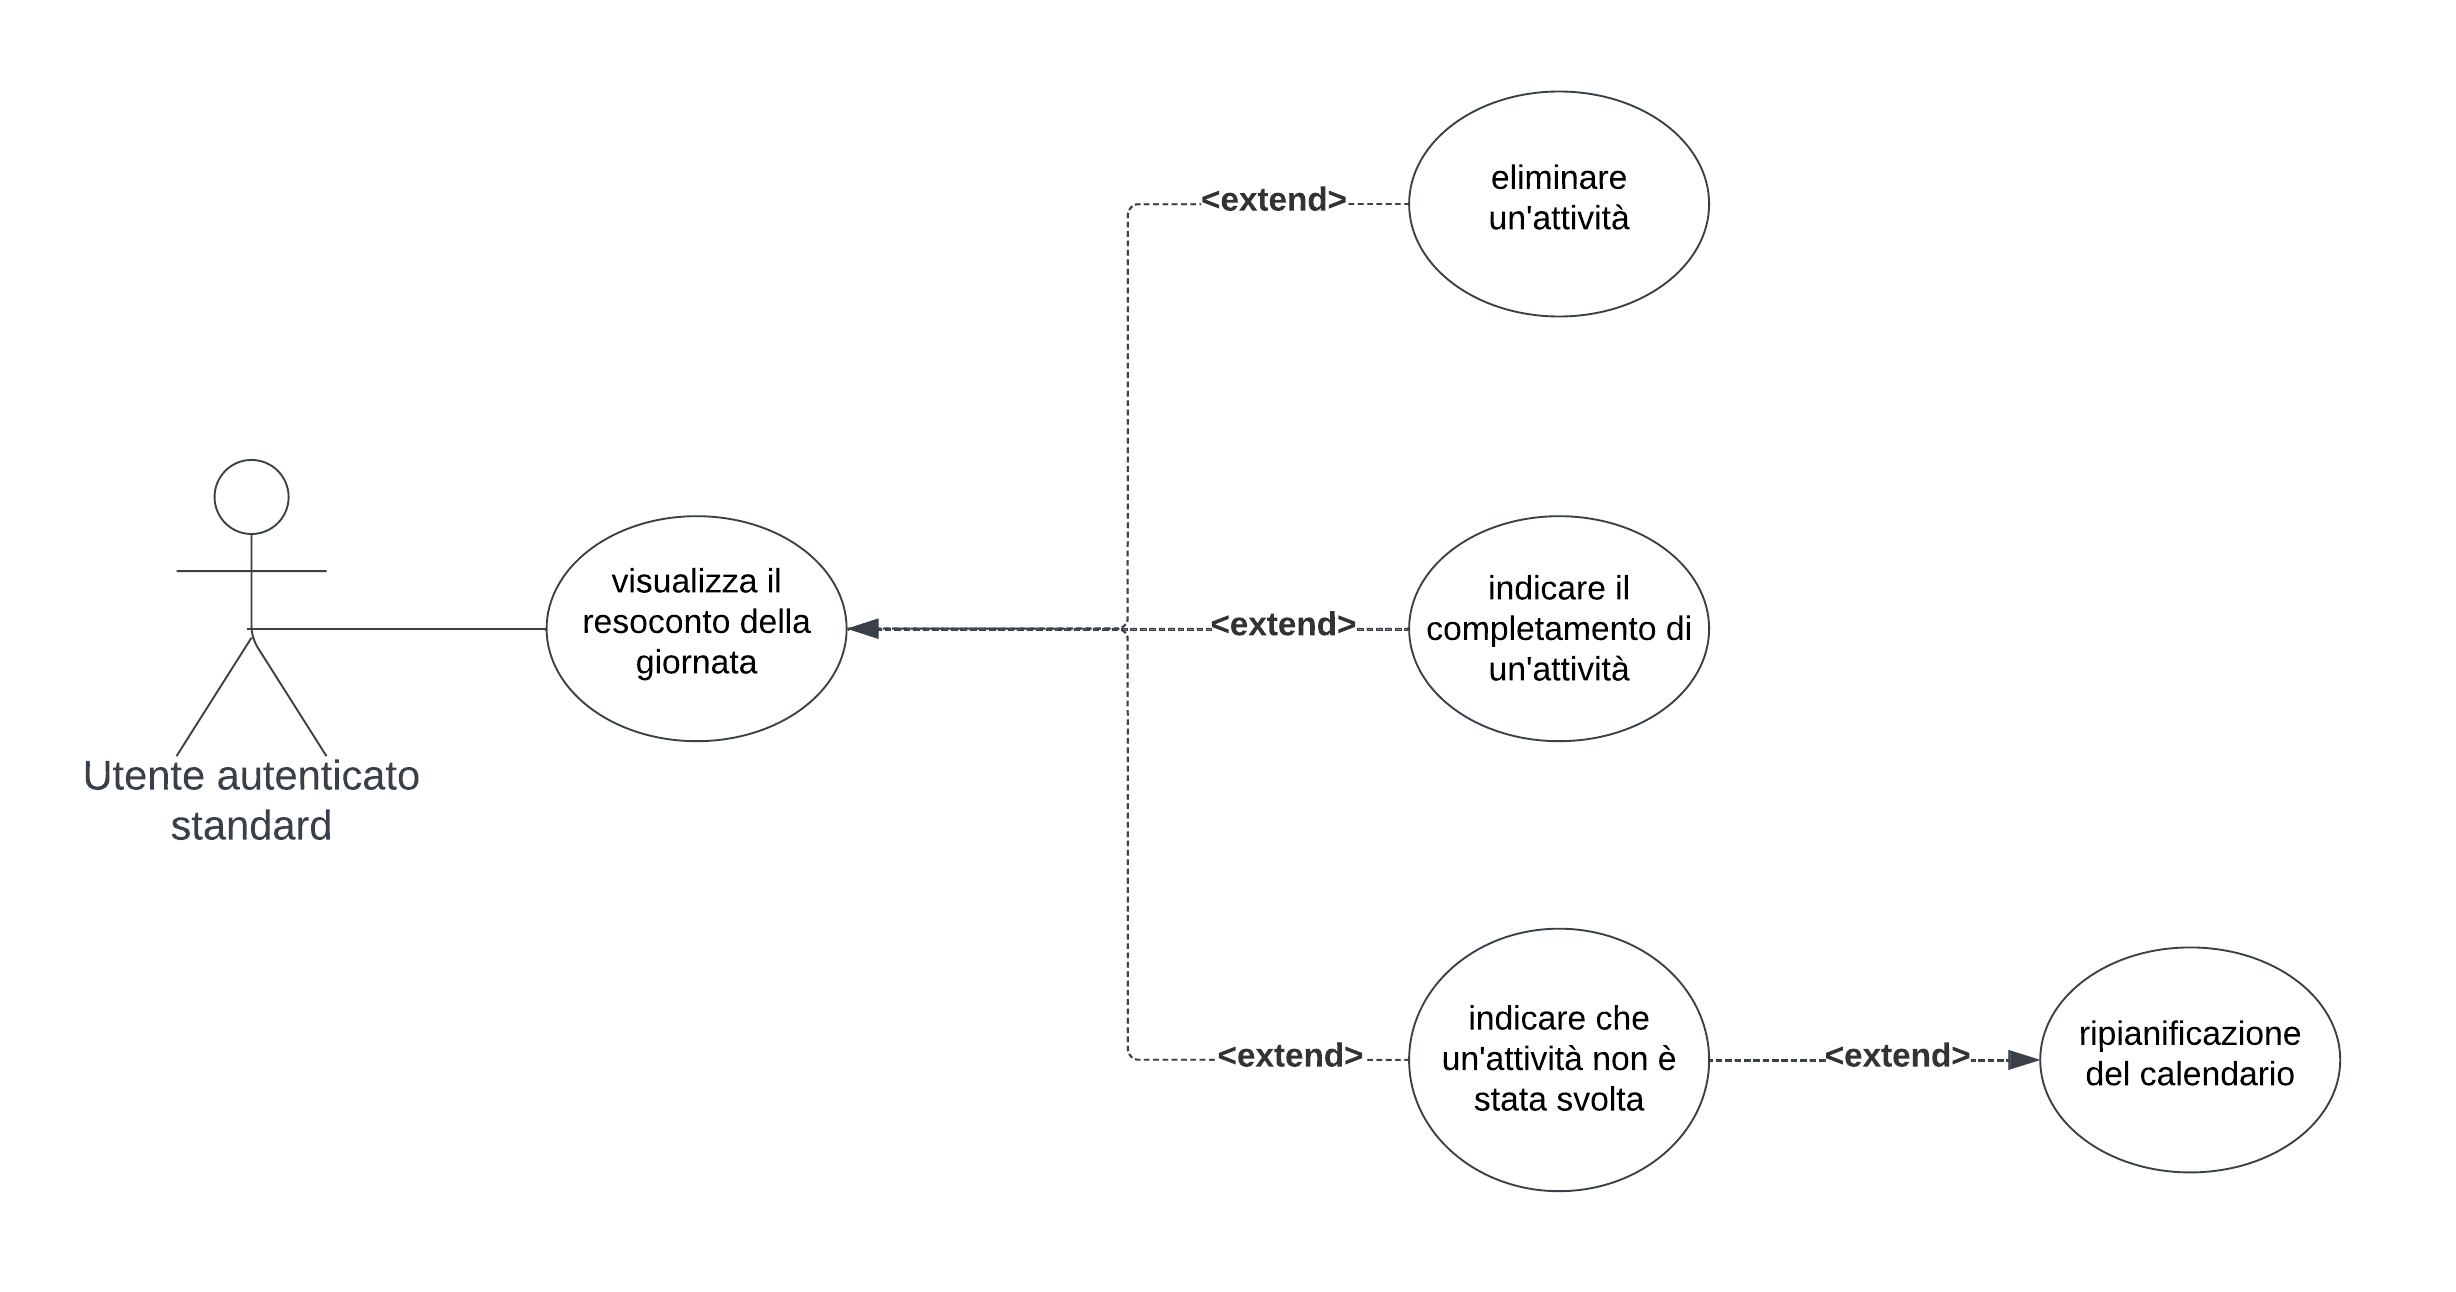
\includegraphics[width=0.7\textwidth]{img/Diagrammi/UseCases/ResocontoGiornata.png}
    \end{center}

    \textbf{Descrizione:}

    \textbf{Riassunto:} questo use case descrive come l'utente autenticato standard visualizza il resoconto della giornata, dove può indicare al sistema quali attività sono state svolte e quali no. Inoltre, in questa sezione, l'utente può anche eliminare le attività. Per resoconto della giornata si intende la lista delle attività della giornata con alcune loro informazioni.

    \textbf{Descrizione:}
    \begin{enumerate}
        \item Nella sezione “Attività”, l'utente autenticato standard visualizza le attività della giornata con alcune loro informazioni, ovvero:
              \begin{itemize}
                  \item titolo;
                  \item descrizione;
                  \item priorità;
                  \item durata;
                  \item posizione;
                  \item difficoltà;
              \end{itemize}
        \item Dalla sezione “Stato” presente in ciascuna attività, l'utente autenticato standard può indicare lo stato dell'attività.
        \item Premendo sulla “spunta”, presente nella sezione “Stato”, questa diviene verde, così l'utente autenticato standard indica il completamento dell'evento, ovvero che è stato svolto. \ref{uc:ExceptionModificaImpegniCompletati}
        \item Premendo sull' “orologio”, presente nella sezione “Stato”, questo diviene giallo, così l'utente autenticato standard indica il non completamento dell'attività. Indicando il non svolgimento di un'attività, il sistema ripianifica il calendario per ridefinire un altro momento dove l'utente può fare questa attività non completata. \ref{uc:ExceptionRipianificazioneAttivitaLibera}
        \item Premendo sul “cestino”, presente nella sezione “Stato”, questo diviene rosso, così l'utente autenticato standard indica l'eliminazione dell'evento dal calendario.
    \end{enumerate}



    \textbf{Exceptions:}
    \begin{enumerate}[label=\textbf{[exception \arabic{enumii}]}, ref= \textbf{[exception \arabic{enumii}]}]
        \elemento{uc:ExceptionModificaImpegniCompletati} A fine giornata di default tutti gli impegni sono posti come completati; quindi per modificare tale “stato” deve intervenire l'utente.
        \elemento{uc:ExceptionRipianificazioneAttivitaLibera} La ripianificazione dell'attività avviene se e solo se l'attività non svolta non aveva definito giorno ed ora dell'impegno. Nel caso in cui fosse un evento per cui l'utente aveva definito giorno ed ora dell'attività in fase di compilazione e aggiunta evento, tale attività non verrà ripianificazione.
    \end{enumerate}

    %\todo{nel FE ordine al contrario della lista non ha molto senso…}





    \newpage
    \elemento[Use case “impostazione delle notifiche per evento”]{uc:ImpostazioniNotifiche}


    \begin{center}
        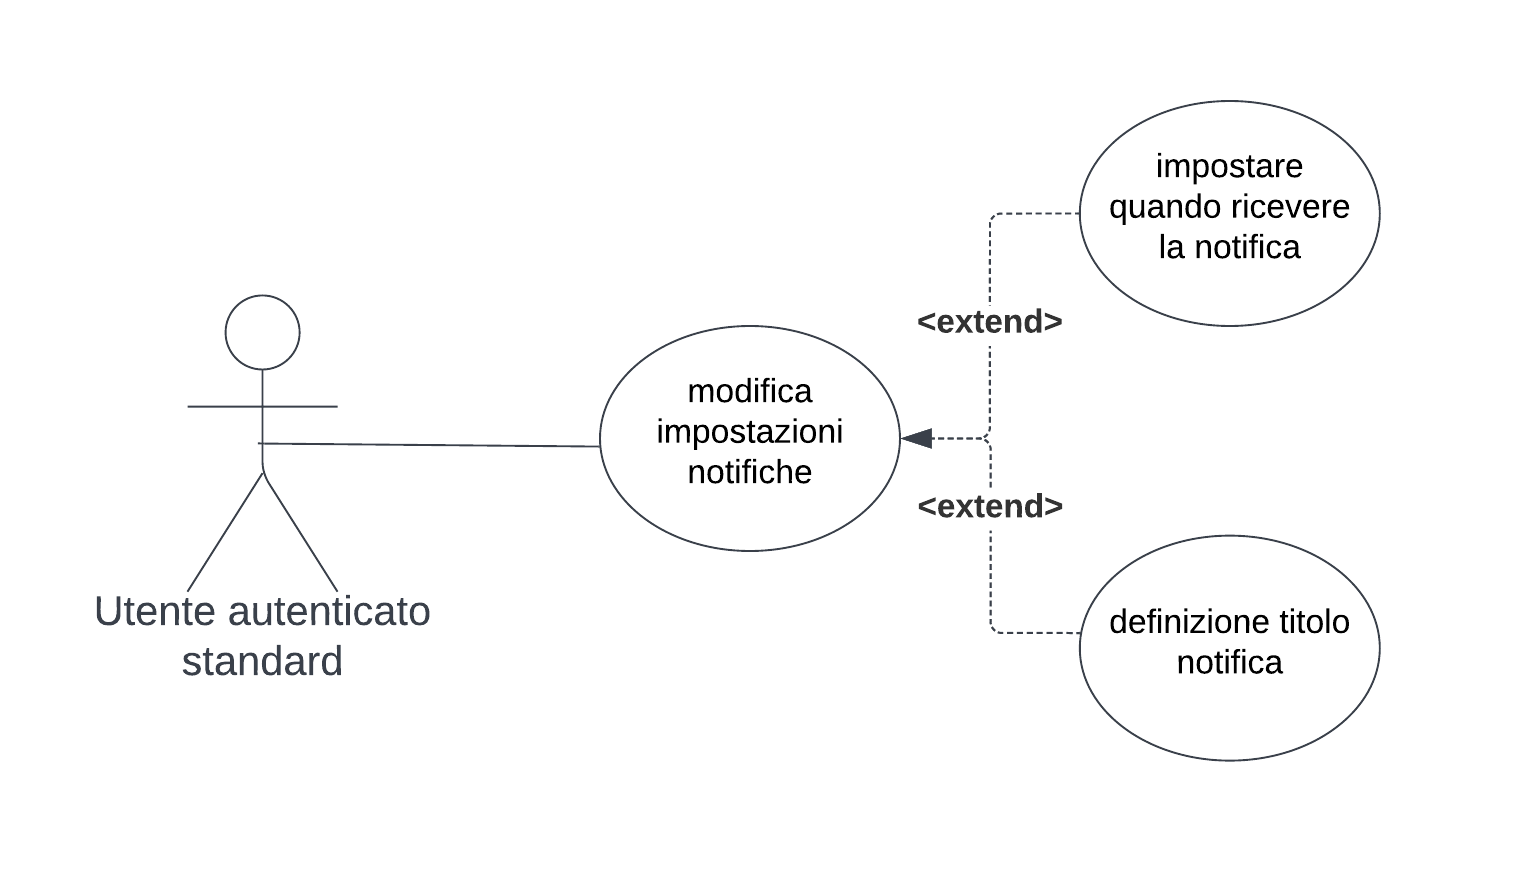
\includegraphics[width=0.7\textwidth]{img/Diagrammi/UseCases/Notifiche.png}
    \end{center}

    \textbf{Descrizione:}

    \textbf{Titolo:} impostazione delle notifiche per evento

    \textbf{Riassunto:}
    Questo use case descrive come avviene l'impostazione delle notifiche per evento. Infatti il sistema dà la possibilità all'utente autenticato standard di personalizzare le notifiche nell'aggiunta e/o modifica dell'evento.

    \textbf{Descrizione:}
    \begin{enumerate}
        \item L'utente autenticato standard dalla schermata “Modifica/Crea Evento” visualizza il menù “Notifiche”.
        \item L'utente autenticato standard premendo sul campo “Notifiche” apre un pop-up dove può definire quando ricevere la notifica dell'evento \ref{uc:ExceptionImpostazioniNotifiche}.
        \item L'utente autenticato standard, sempre nel pop-up, può inserire il titolo della notifica che riceverà \ref{uc:ExceptionImpostazioniNotifiche}.
    \end{enumerate}

    \textbf{Exceptions:}
    \begin{enumerate}[label=\textbf{[exception \arabic{enumii}]}, ref= \textbf{[exception \arabic{enumii}]}]
        \elemento{uc:ExceptionImpostazioniNotifiche} Nel caso in cui l'utente autenticato standard decidesse di non modificare i campi presenti in “Notifiche” verrà mantenuto il valore definito nelle impostazioni predefinite del calendario, ovvero:
        \begin{itemize}
            \item la notifica verrà mandata tanto prima quanto indicato nell'impostazione predefinita del calendario in cui stiamo aggiungendo tale evento;
            \item la notifica avrà come titolo, il titolo dell'evento stesso.
        \end{itemize}
    \end{enumerate}


    %\todo{forse potrei mettere utente autenticato senza standard, così per inglobare meglio quello premium ma credo che così vada bene, visto che abbiamo specificato che l'utente premium prende tutte le funzionalità da quello standard}




    \newpage
    \elemento[Use case “interazione con Google Calendar”]{uc:GoogleCalendar}


    \begin{center}
        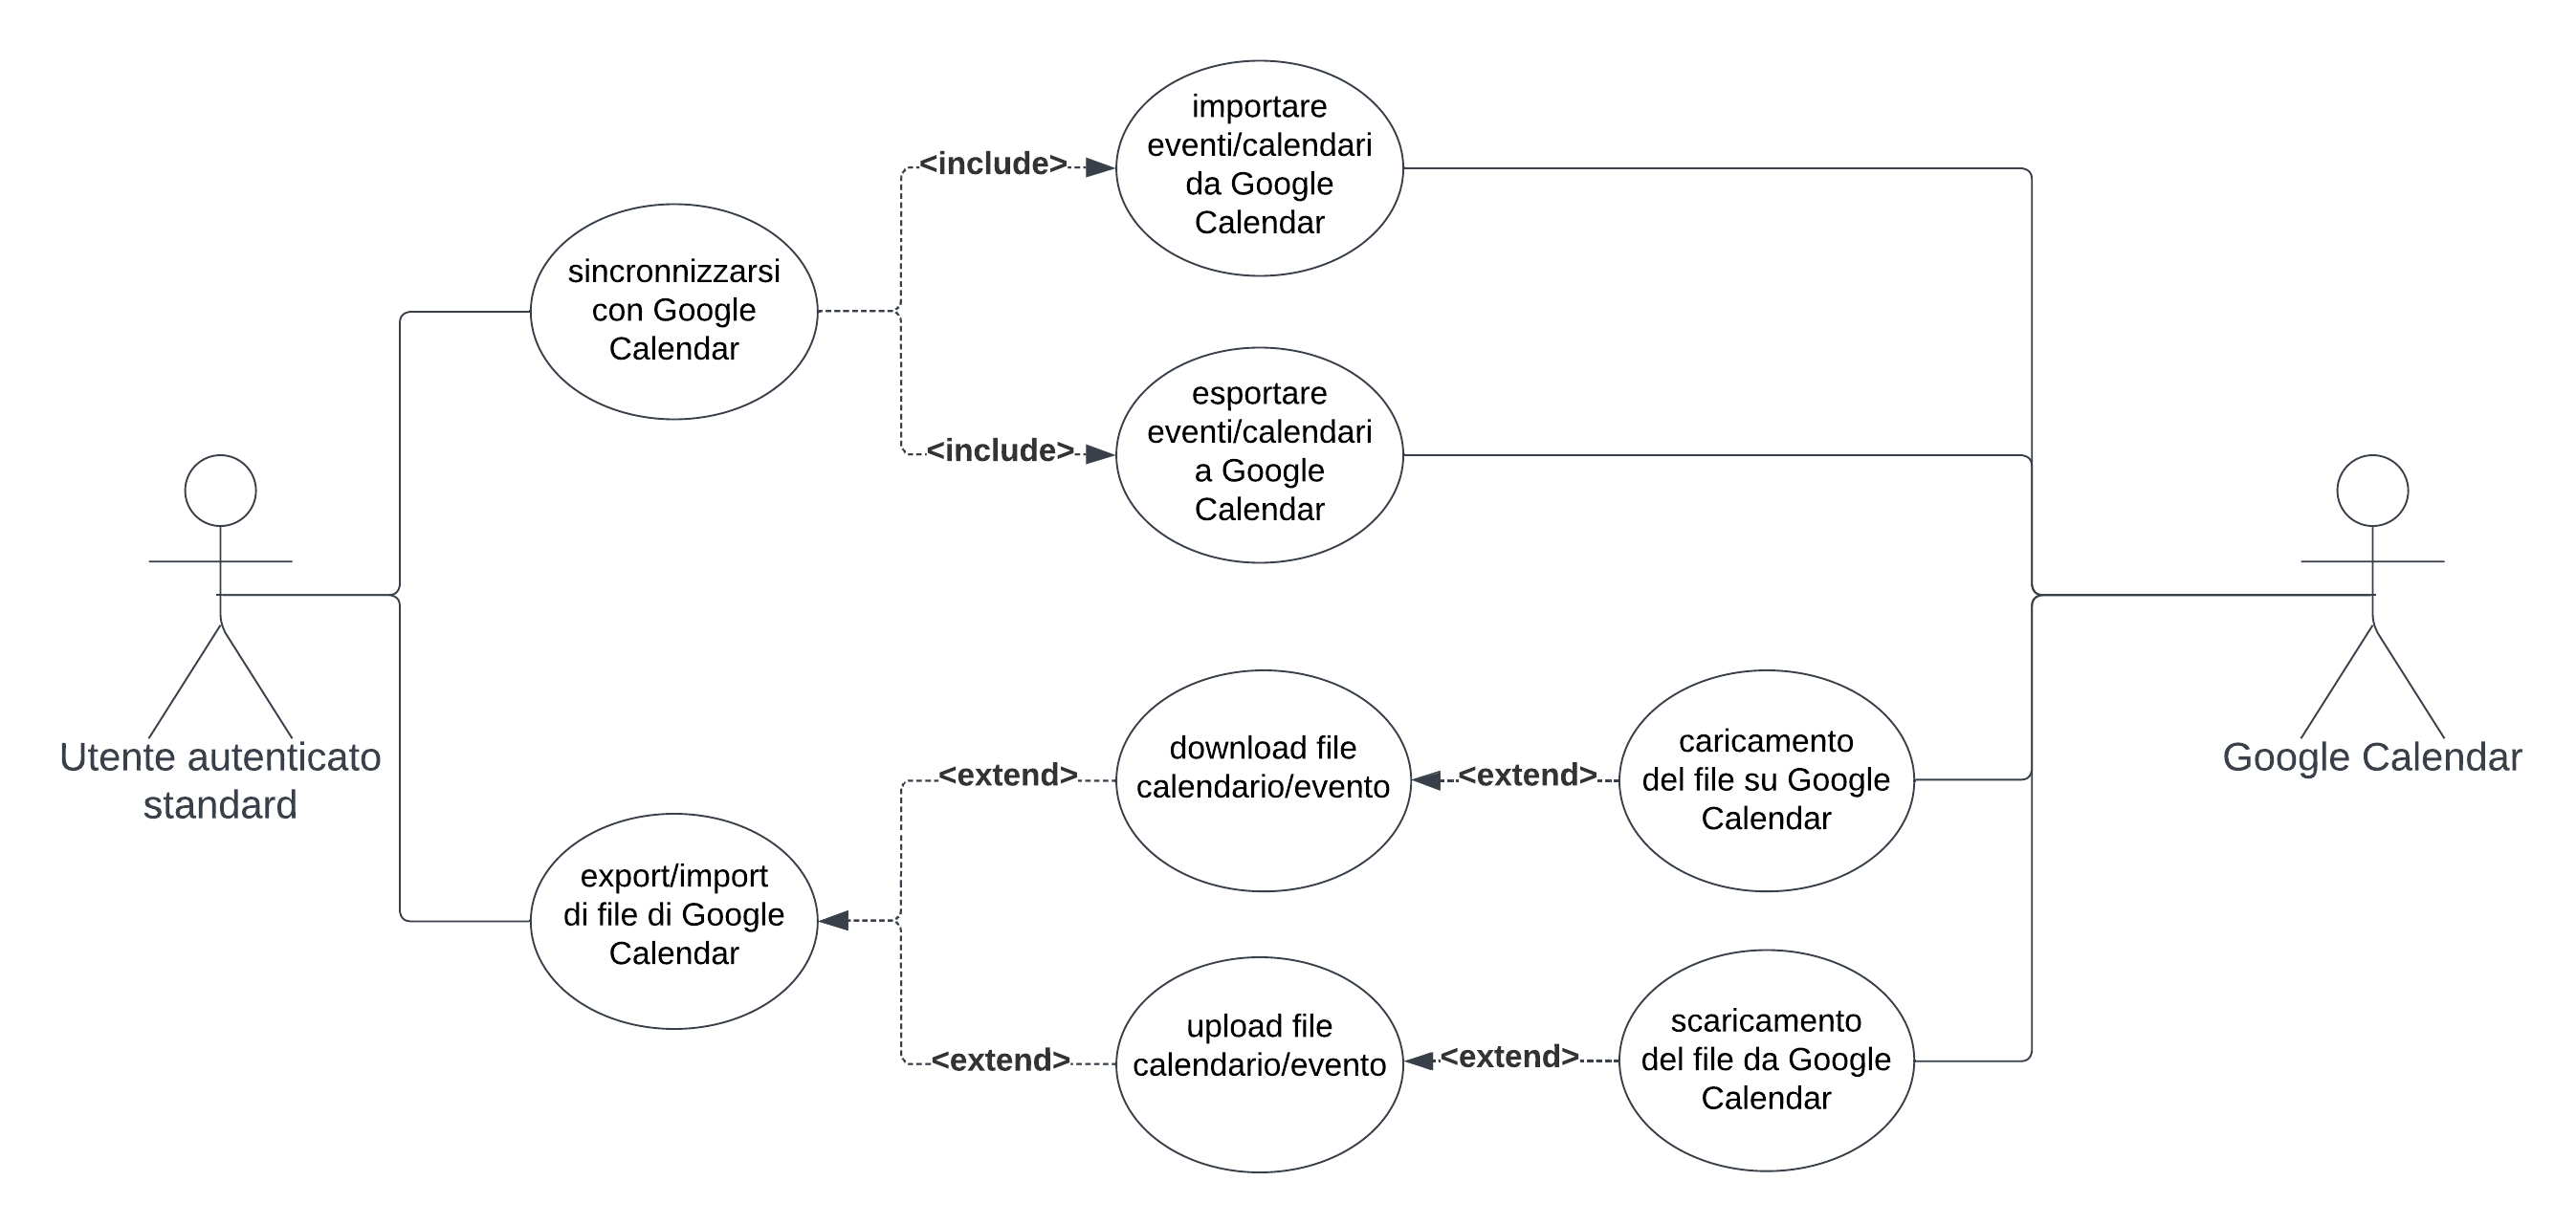
\includegraphics[width=0.8\textwidth]{img/Diagrammi/UseCases/GoogleCalendar.png}
    \end{center}

    \textbf{Descrizione:}

    \textbf{Titolo:} interazione con Google Calendar.

    \textbf{Riassunto:}
    Questo use case descrive come il sistema permetta all'utente autenticato standard l'utilizzo di Google Calendar dalla piattaforma. Infatti, in quanto Google Calendar è un'applicazione molto diffusa, il sistema permette l'interazione con questa applicazione.

    \textbf{Descrizione:}
    \begin{enumerate}
        \item L'utente autenticato standard potrà decidere se connettere il proprio account Google Calendar al proprio account. Ciò avverrà tramite un'apposita finestra di dialogo dove l'utente autenticato standard farà l'accesso al proprio account Google e concederà alla piattaforma i permessi di interagire con il calendario \ref{uc:ExceptionInterruzioneSincronizzazione}. Una volta concessa l'autorizzazione si potrà scegliere quale calendario sincronizzare, se sincronizzare gli eventi da e/o verso Google Calendar.
        \item In alternativa nella sezione “importa/esporta” della piattaforma si potrà trovare un modo per esportare \ref{uc:ExceptionErroreDownload} su file il proprio calendario e un modo per poter caricare un file \ref{uc:ExceptionErroreUpload} per importare un calendario preesistente sulla piattaforma.
    \end{enumerate}

    \textbf{Exceptions:}
    \begin{enumerate}[label=\textbf{[exception \arabic{enumii}]}, ref= \textbf{[exception \arabic{enumii}]}]
        \elemento{uc:ExceptionInterruzioneSincronizzazione} Nel caso in cui l'utente autenticato standard decidesse di interrompere la procedura di autenticazione/gestione consensi l'attività di importazione/esportazione non andrà a termine.
        \elemento{uc:ExceptionErroreUpload} Nel caso l'utente autenticato standard non finisse di caricare il file, il calendario da file caricato non potrà essere caricato sulla piattaforma in quanto mancherebbero informazioni.
        \elemento{uc:ExceptionErroreDownload} Se dopo aver richiesto alla piattaforma di esportare il proprio calendario su file si chiude la piattaforma prima di iniziare il download del file, lo scaricamento del file non avverrà.
    \end{enumerate}

    %\todo{Forse bisogna cambiare l'importazione esportazione automatica in sincronizzazione nel Diagramma}



    \newpage
    \elemento[Use case “Informazioni sull'uso del tempo”]{uc:InformazioniUsoDelTempo}


    \begin{center}
        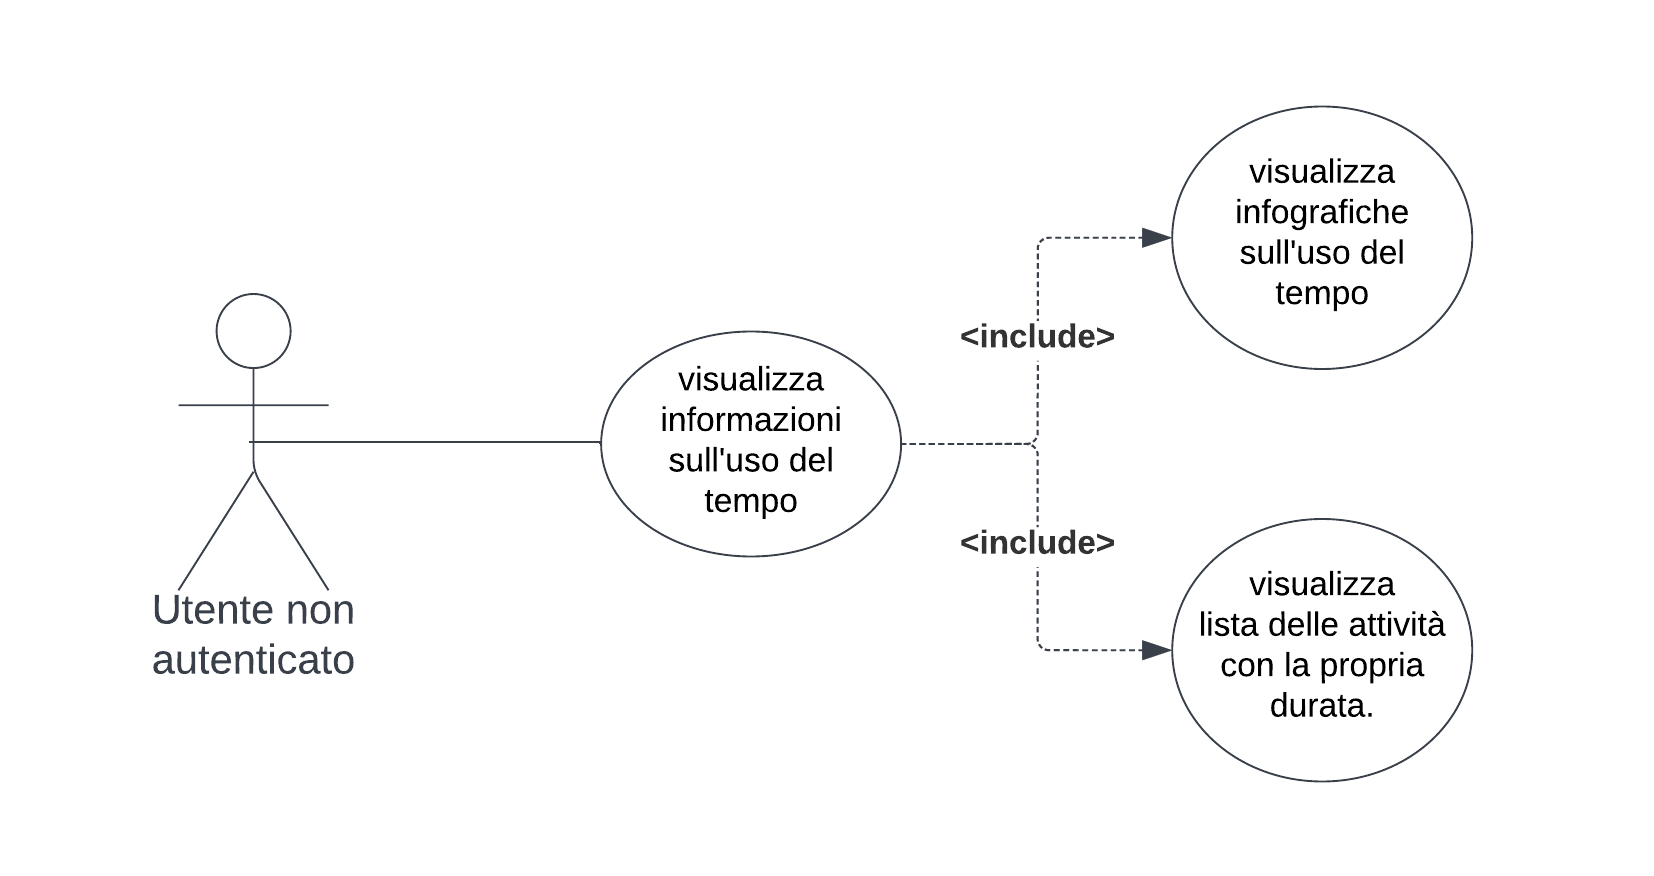
\includegraphics[width=0.7\textwidth]{img/Diagrammi/UseCases/UsoDelTempo.png}
    \end{center}

    \textbf{Descrizione:}

    \textbf{Titolo:} informazioni sull'uso del tempo

    \textbf{Riassunto:} questo use case descrive come l'utente non autenticato può visualizzare dei grafici e liste esemplificative sull'uso del proprio tempo.

    \textbf{Descrizione:}
    \begin{enumerate}
        \item L'utente non autenticato dalla sezione Dashboard visualizza delle infografiche:
              \begin{itemize}
                  \item un grafico a barre dei vari eventi per ogni giorno della settimana; l'altezza delle barre corrisponde al quantitativo di ore dedicate a quell'attività. \ref{uc:ExtensionSelezioneAttivita}
                  \item una heatmap riguardo al tempo che deve essere dedicato ogni giorno per rispettare le varie deadline.
                  \item un grafico a torta delle attività. La dimensione di ciascuna attività, all'interno del grafico a torta,ha una dimensione proporzionata al tempo da spendere.
              \end{itemize}
        \item L'utente non autenticato , in questa sezione, visualizza anche una lista delle attività del proprio calendario, che è sincronizzata con il grafico a torta sopra citato, ovvero nelle due sezioni sono presenti le stesse attività con le medesime durante. \ref{uc:ExtensionSincronizzazioneGrafici} \ref{uc:ExtensionVisualizzazioneAttivita}
    \end{enumerate}

    \textbf{Extensions:}
    \begin{enumerate}[label=\textbf{[extension \arabic{enumii}]}, ref= \textbf{[extension \arabic{enumii}]}]
        \elemento{uc:ExtensionSelezioneAttivita} Selezionando un' attività dalla legenda del grafico, il grafico evidenzia l'attività selezionata in modo tale che l'utente non autenticato possa vedere meglio quando ha tale evento.
        \elemento{uc:ExtensionSincronizzazioneGrafici} La sincronizzazione tra grafico a torta e lista di attività si mantiene anche in caso di modifiche temporanee della lista di attività. Infatti premendo su un'attività, il sistema modifica la lista delle attività mostrando le sottoattività di quest'ultima e aggiornando il grafico a torta secondo la nuova lista visualizzata.
        \elemento{uc:ExtensionVisualizzazioneAttivita} Mettendo il cursore sopra ad una delle attività della lista, l'utente non autenticato visualizza evidenziata tale attività nel grafico a torta.
    \end{enumerate}



    \newpage
    \elemento[Use case “Filtro impegni”]{uc:FiltroImpegni}


    \begin{center}
        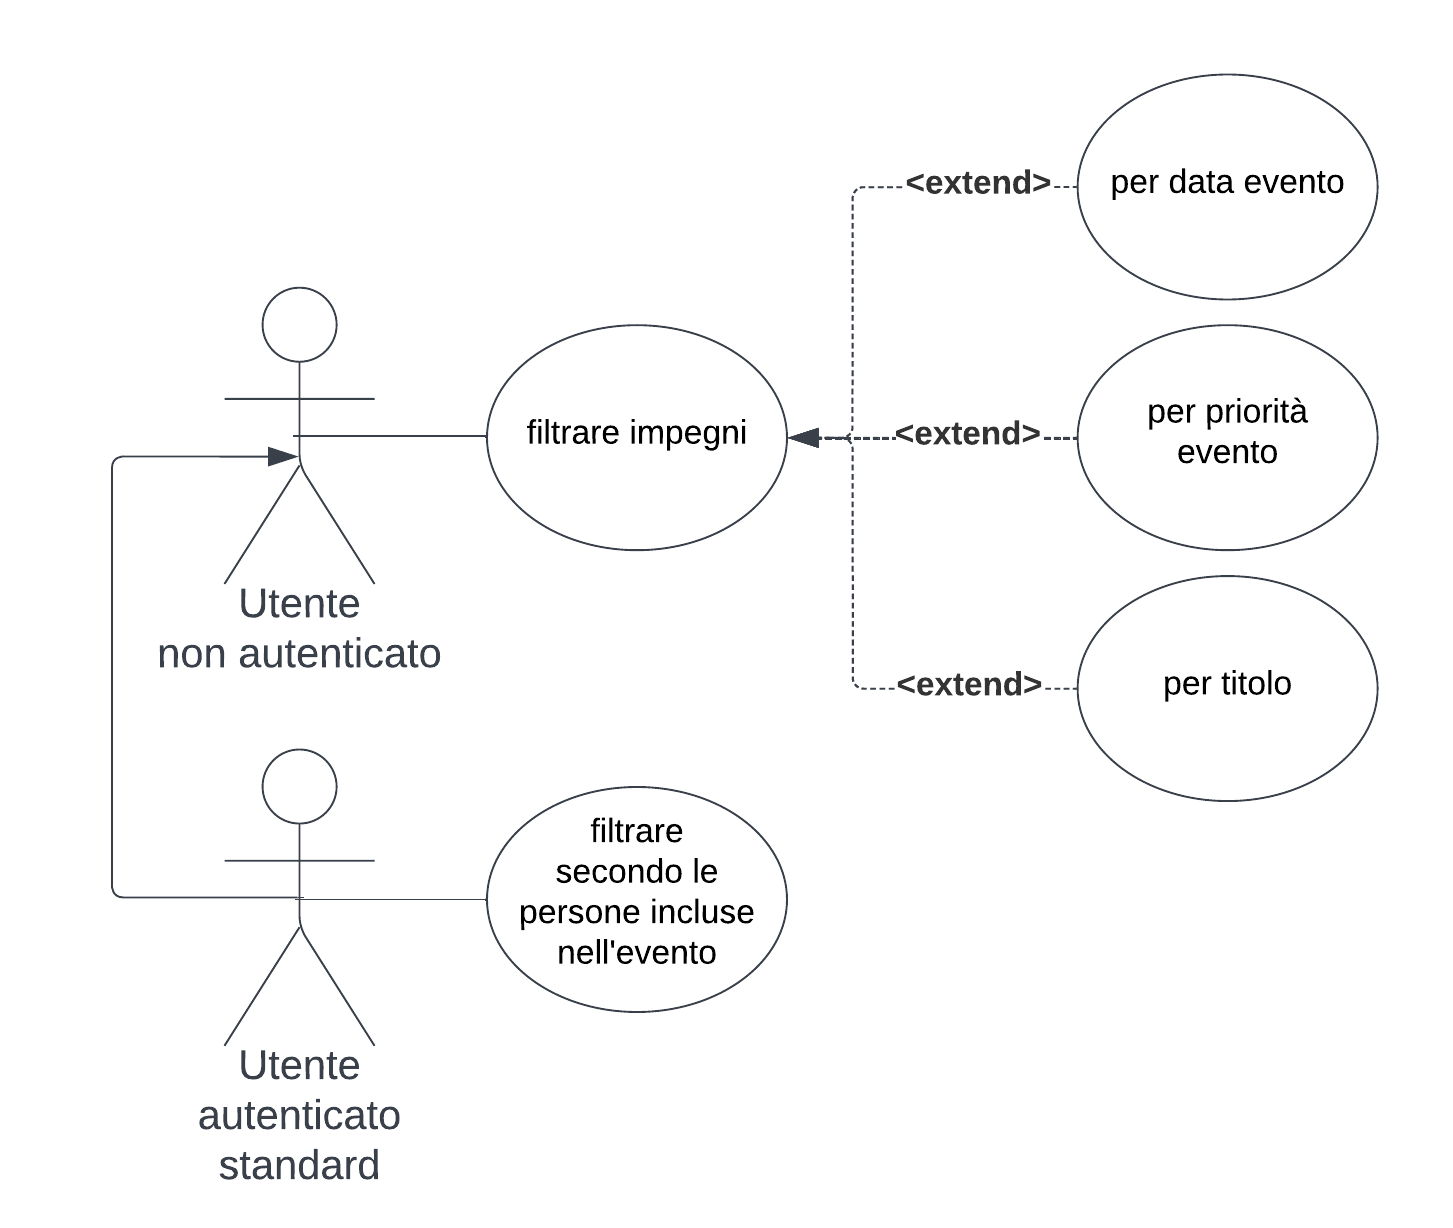
\includegraphics[width=0.7\textwidth]{img/Diagrammi/UseCases/Filtro.png}
    \end{center}

    \textbf{Descrizione:}

    \textbf{Titolo:} filtro impegni

    \textbf{Riassunto:} questo use descrive come l'utente non autenticato visualizza gli impegni dato un specifico filtro definito secondo alcuni criteri scelti dall'utente non autenticato.

    \textbf{Descrizione:}
    \begin{enumerate}
        \item Nelle sezione “Filtro” l'utente può visualizzare gli impegni dato un specifico filtro definito dall'utente secondo alcuni criteri:
              \begin{itemize}
                  \item titolo evento con corrispondenza totale o parziale;
                  \item data evento;
                  \item priorità evento;
                  \item persone include nell'evento;
              \end{itemize}
        \item L'utente può definire secondo quali valori dei criteri andare a filtrare gli impegni andando a scrivere nelle caselle di ciascun criterio, visualizzabili in questa sezione “FIltro”. \ref{uc:ExceptionNienteCriterioFiltro}
        \item Dopo aver definito i criteri degli impegni da visualizzare, l'utente premendo il tasto di ricerca visualizzerà, in un pop-up, la lista delle attività che rispettano i criteri imposti dall'utente.

              %\todo{(potremmo anche mettere che questi appaiono direttamente nel calendario)}
    \end{enumerate}

    \textbf{Exceptions:}
    \begin{enumerate}[label=\textbf{[exception \arabic{enumii}]}, ref= \textbf{[exception \arabic{enumii}]}]
        \elemento{uc:ExceptionNienteCriterioFiltro} Nel caso in cui l'utente non andasse a definire il valore di uno o più criteri, i valori che verranno presi in considerazione per filtrare le attività sono tutti i valori che può assumere un criterio. Per esempio, se l'utente non andasse a definire il valore del criterio priorità, nel filtrare gli impegni verranno prese in considerazioni tutte le priorità, quindi da 1 a 10.
    \end{enumerate}

    %\todo{In quale sezione sarà presente il filtro impegni? e come sarà gestito? Apparirà una lista delle attività delle attività che rispettano i criteri posti, oppure questi appariranno nel calendario (schermata principale). da mettere nel FE}



    \newpage
    \elemento[Use case “Creazione e modifica di un calendario”]{ud:CreazioneModificaCalendario}


    \begin{center}
        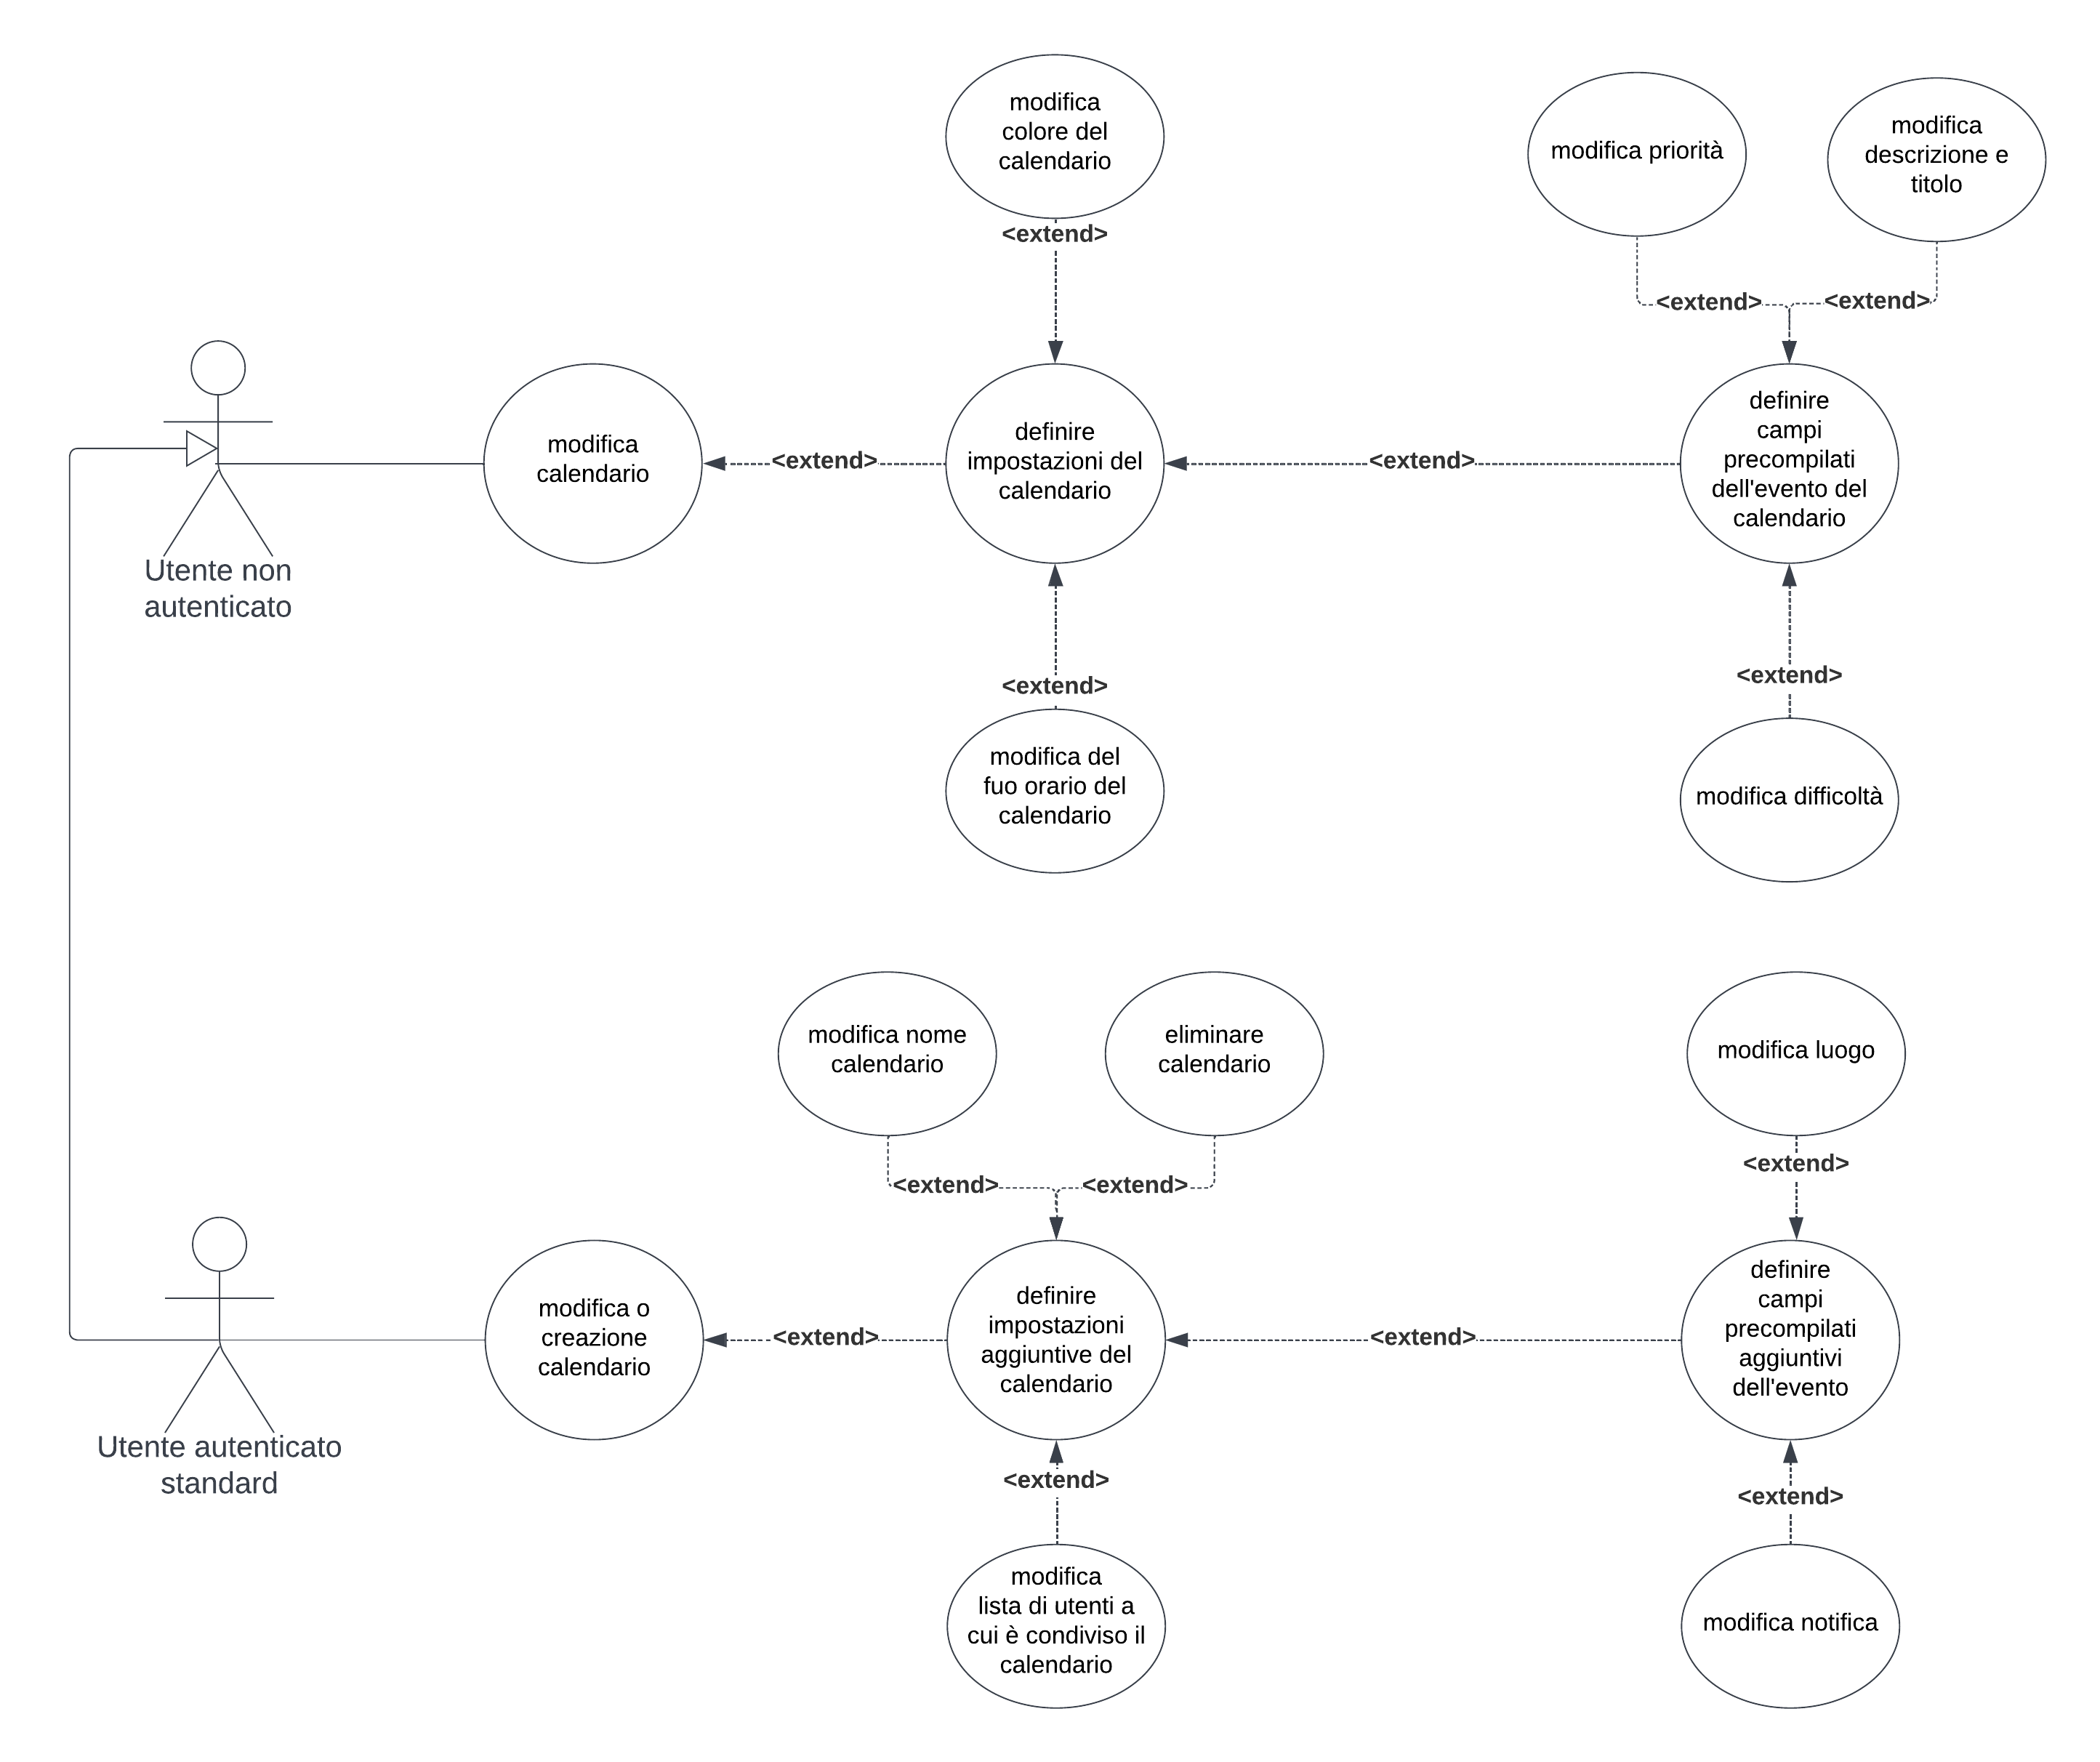
\includegraphics[width=1\textwidth]{img/Diagrammi/UseCases/ImpostazioniPredefiniteCalendario.png}
    \end{center}

    \textbf{Descrizione:}

    \textbf{Titolo:} creazione e modifica delle impostazioni predefinite di un calendario

    \textbf{Riassunto:} questa use case descrive come l'utente non autenticato può andare a modificare impostazioni del calendario principale. Queste impostazioni saranno anche usate per precompilare i campi dell'evento quando si va ad aggiungerlo. Inoltre questo use case descrive anche come l'utente autenticato standard può andare a creare o modificare un calendario avendo delle impostazioni aggiuntive rispetto all'utente non autenticato.

    \textbf{Descrizione:}
    \begin{enumerate}
        \item L'utente non autenticato dalla sezione  “Impostazioni predefinite di un calendario” può andare a modificare le impostazioni del proprio calendario principale. Nello specifico, in questa sezione sono presenti i seguenti campi in cui può andare a scrivere per modificare i loro valori:
              \begin{itemize}
                  \item colore del calendario,
                        %\todo{ ovvero il colore con cui appariranno gli eventi appartenenti a quest'ultimo.}
                  \item fuso orario del calendario;
              \end{itemize}
        \item L'utente non autenticato può anche definire dei valori di default dei seguenti campi, presenti nella compilazione dell'evento da aggiungere al calendario principale: \ref{ud:ExceptionCampiPrecompilatiCalendario}:
              \begin{itemize}
                  \item priorità;
                  \item descrizione e titolo;
                  \item difficoltà, ovvero la complessità dell'evento da svolgere;
              \end{itemize}
        \item L'utente non autenticato salva le modifiche fatte premendo il tasto “Salva” in fondo alla schermata di “Impostazioni predefinite di calendario”. Invece, premendo il tasto “Annulla”, le modifiche fatte non verranno salvate.
        \item L'utente autenticato standard, oltre alla possibilità sopra citate per l'utente non autenticato ha altre funzionalità, ovvero:
              \begin{itemize}
                  \item creazione e modifica di più calendari personali;
                  \item impostazioni aggiuntive per i calendari;
                  \item campi precompilati aggiuntivi nella compilazione dell'evento.
              \end{itemize}
        \item Nella sezione “Eventi”, selezionando “Crea Calendario” l'utente autenticato standard apre la schermata di creazione di un calendario.
        \item In questa schermata, l'utente può andare a definire delle impostazioni riguardanti al calendario che sta creando, ovvero:
              \begin{itemize}
                  \item tutti i campi già presenti per la modifica del calendario principale per un utente non autenticato, ovvero nome, colore, fuso orario del calendario.
                  \item persone a cui sarà condiviso il calendario;
              \end{itemize}
        \item L'utente può anche definire dei valori di default dei seguenti campi presenti nella compilazione dell'evento da aggiungere: \ref{ud:ExceptionCampiPrecompilatiCalendario}
              \begin{itemize}
                  \item tutti i campi già presenti per la definizione di valori di default nella compilazione di un evento da parte dell'utente non autenticato, ovvero descrizione e titolo, difficoltà e priorità;
                  \item luogo dove si terrà;
                  \item quando ricevere la notifica dell'evento;
                  \item titolo della notifica dell'evento.
              \end{itemize}
        \item L'utente autenticato standard, così, può creare il calendario premendo il tasto “Salva” che si trova in fonda alla schermata. L'utente può annullare l'azione premendo il tasto “Annulla” che trova sempre in fondo alla schermata di “Crea Calendario”.
        \item Tutti campi sopra citati, presenti nella schermata “Crea Calendario”, sono presenti anche nella sezione “Impostazioni predefinite di un calendario” per un utente autenticato standard, dove l'utente autenticato standard può sempre andare a modificare questi campi secondo le proprie preferenze. L'utente autenticato standard deve selezionare il calendario, di cui vuole modificare le impostazioni, dalla lista dei propri calendari, presente nella parte sinistra di questa schermata.
    \end{enumerate}

    \textbf{Exceptions:}
    \begin{enumerate}[label=\textbf{[exception \arabic{enumii}]}, ref= \textbf{[exception \arabic{enumii}]}]
        \elemento{ud:ExceptionCampiPrecompilatiCalendario} Nel caso in cui l'utente non modificasse uno o più campi, nella compilazione per l'aggiunta di un evento l'utente non visualizzerà precompilati i campi non modificati nelle “Impostazioni predefinite di un calendario”.
    \end{enumerate}





    \newpage
    \elemento[Use case “Impostazioni account”]{uc:ImpostazioniAccount}

    \begin{center}
        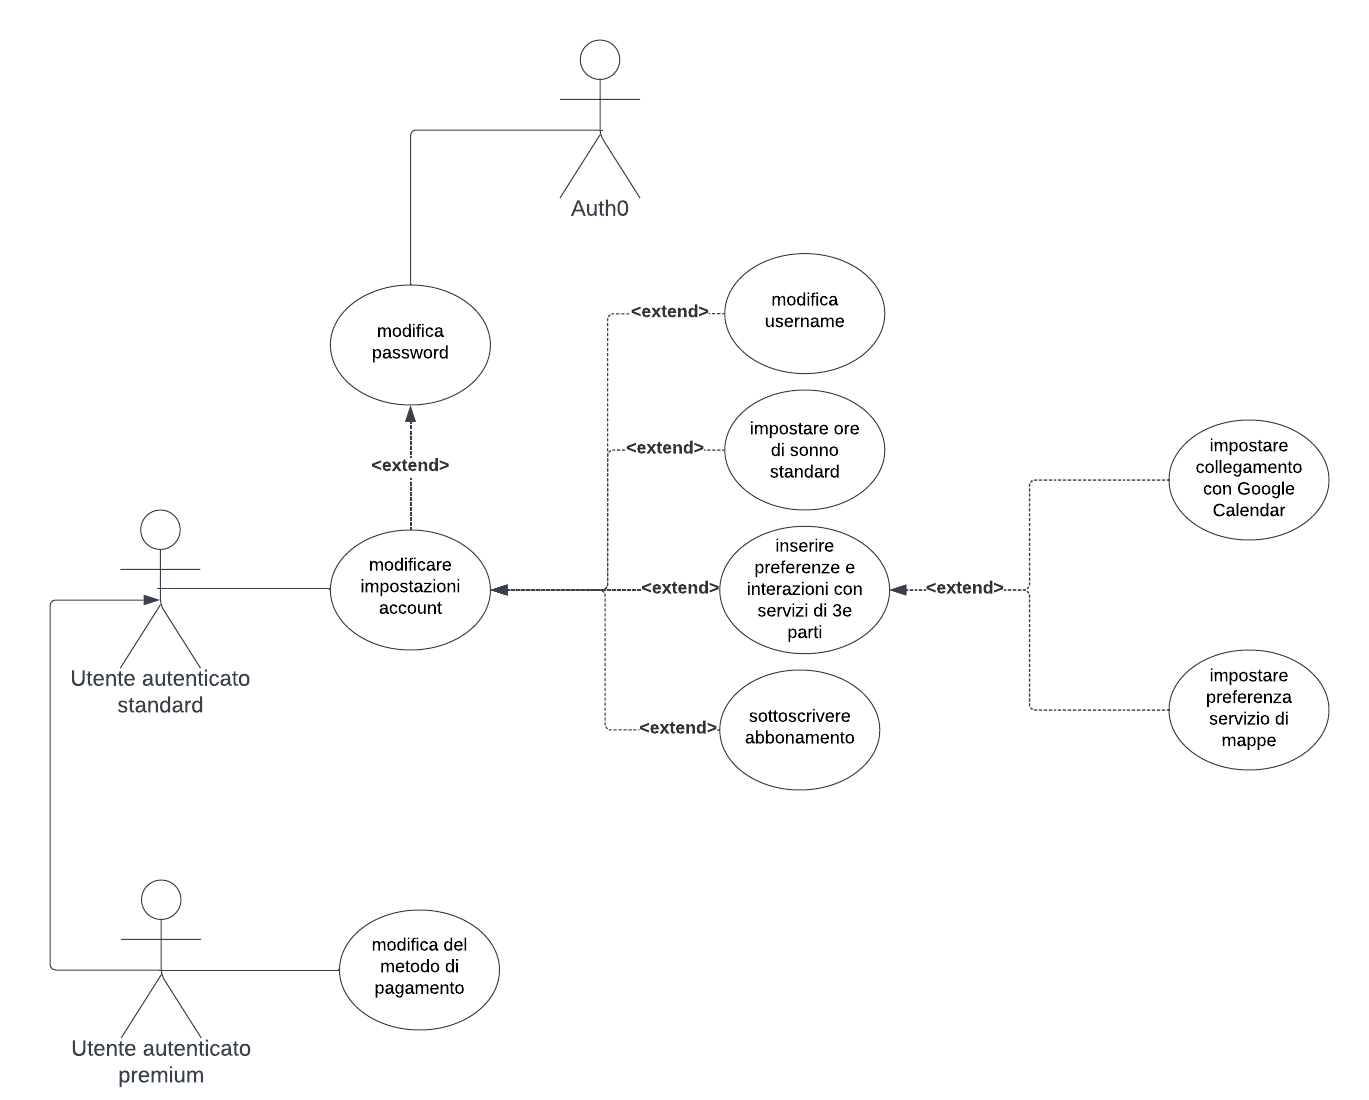
\includegraphics[width=0.7\textwidth]{img/Diagrammi/UseCases/ImpostazioniAccount.png}
    \end{center}


    \textbf{Diagramma:}
    \begin{center}
        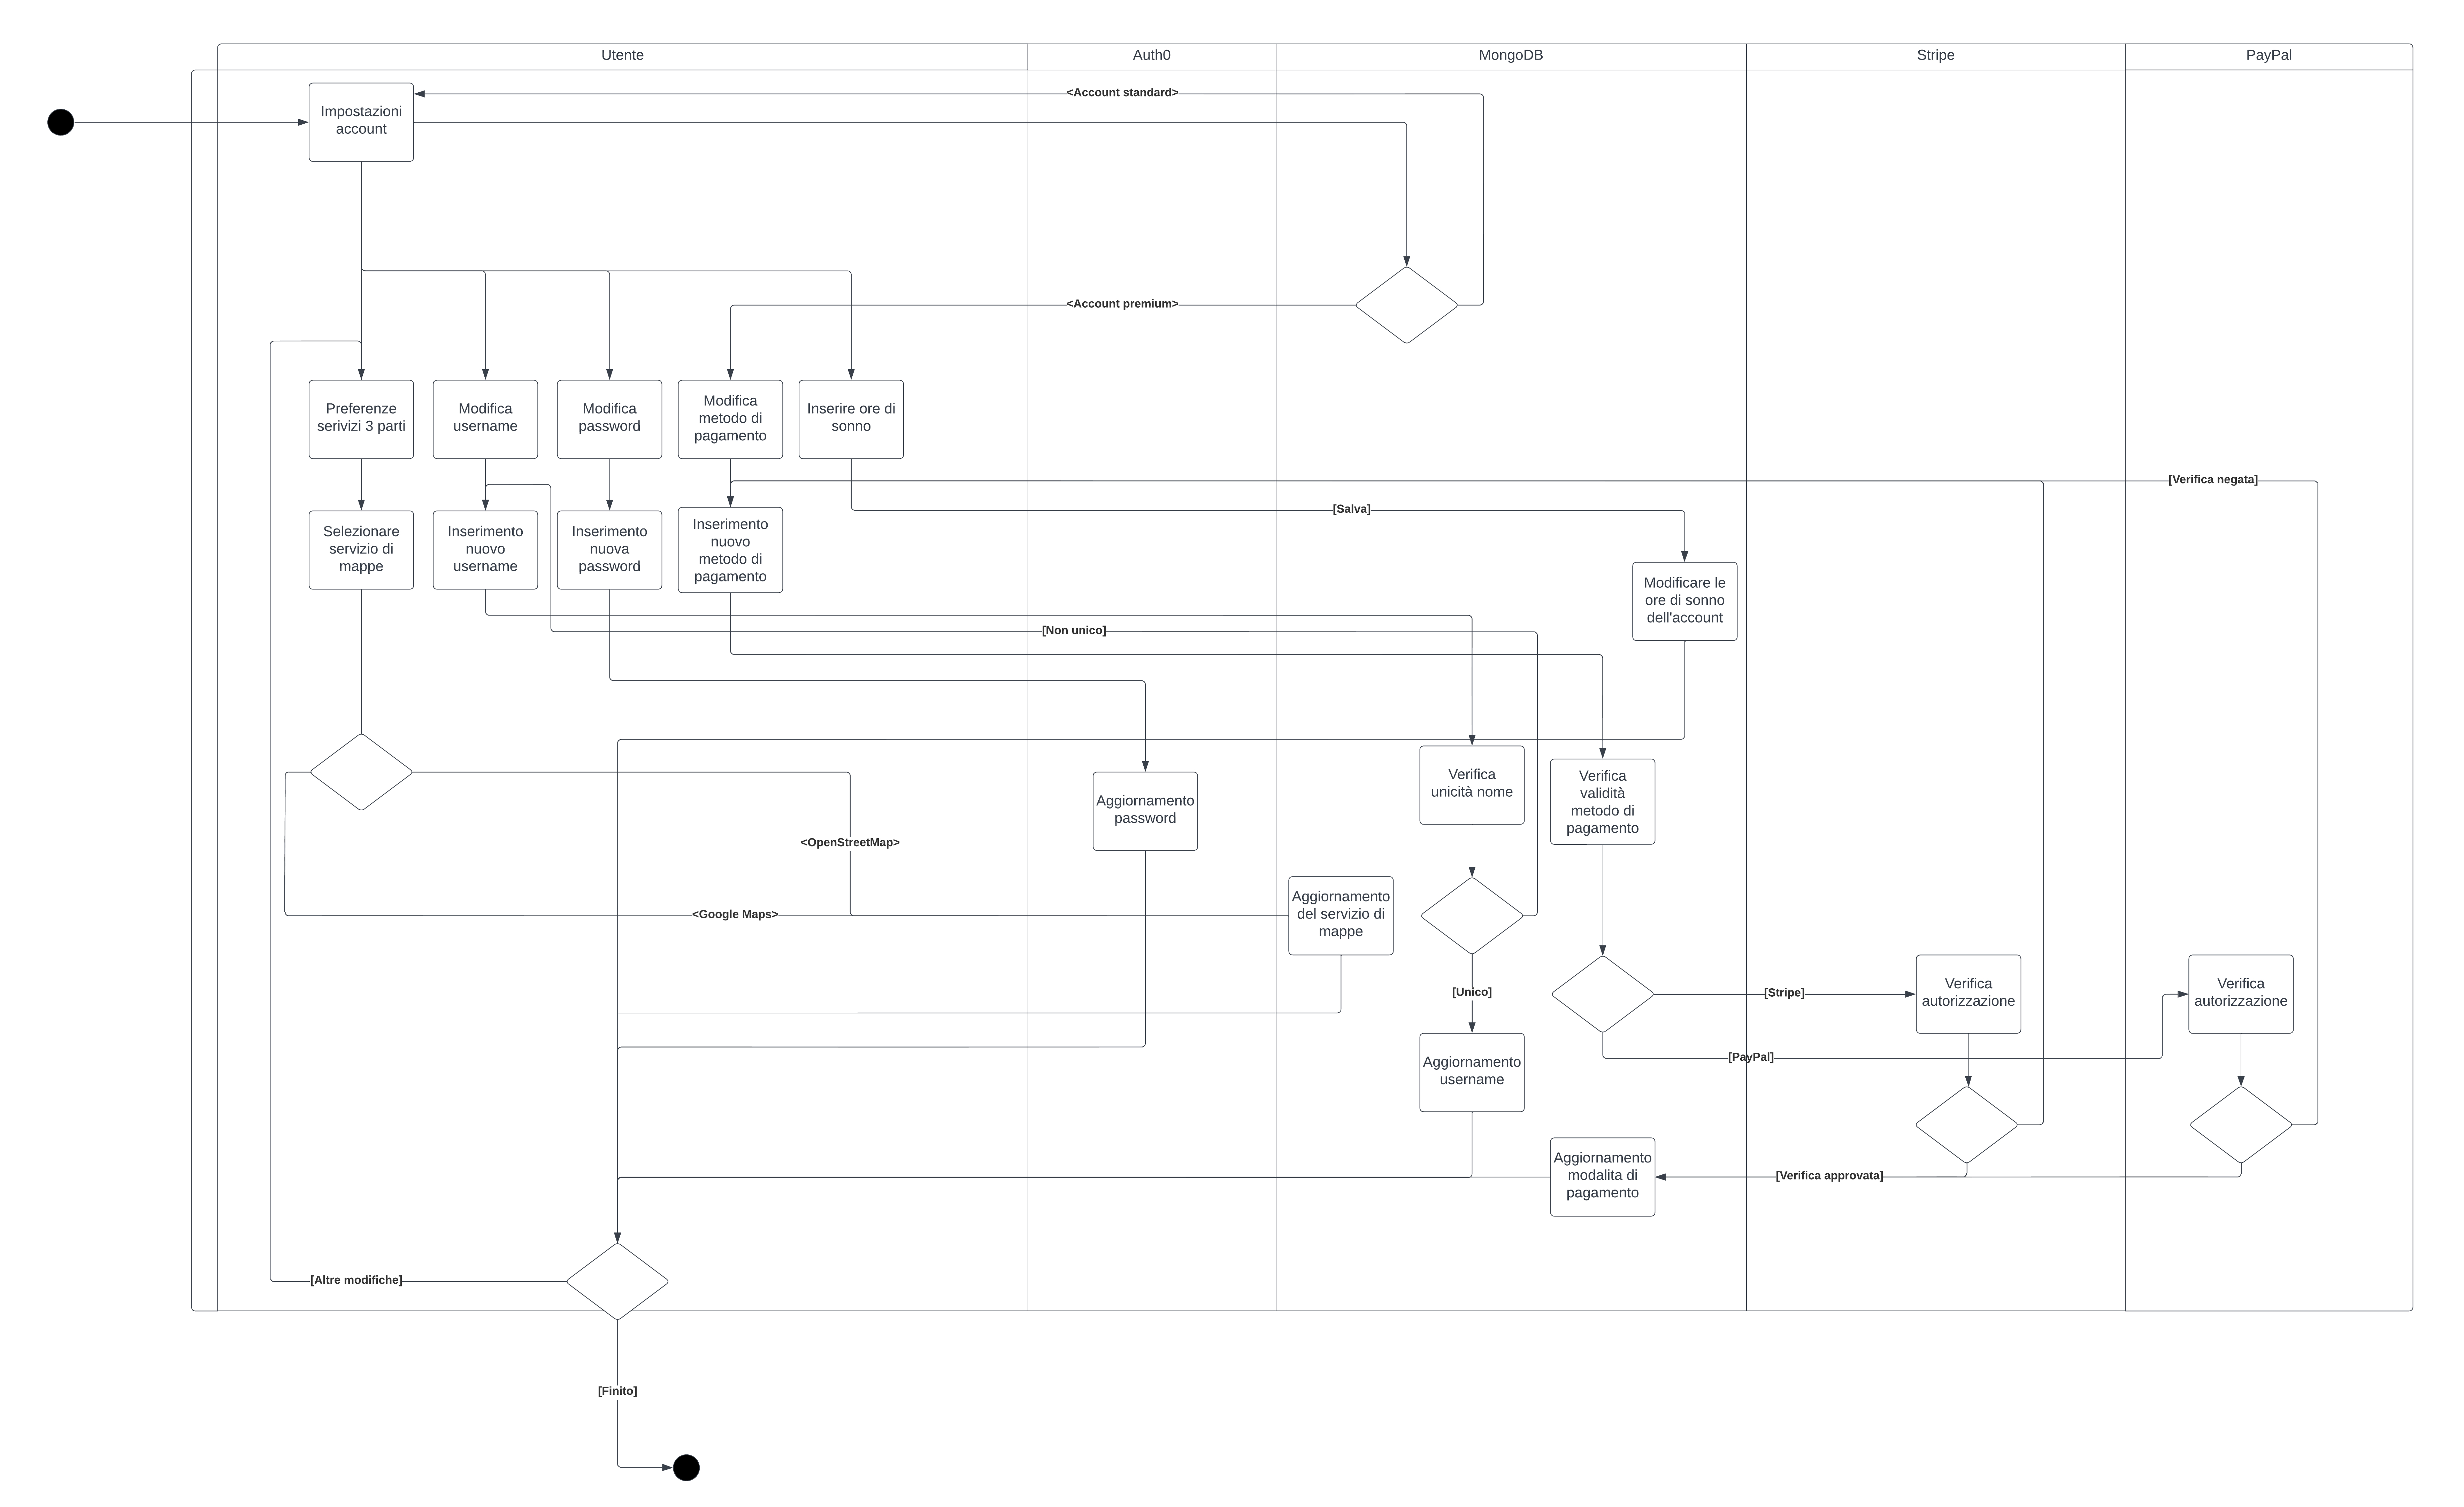
\includegraphics[width=1\textwidth]{img/Diagrammi/DS/DS_ImpostazioneAccount.png}
    \end{center}




    \newpage
    \elemento[Use case “Recupero password”]{uc:RecuperoPassword}

    \begin{center}
        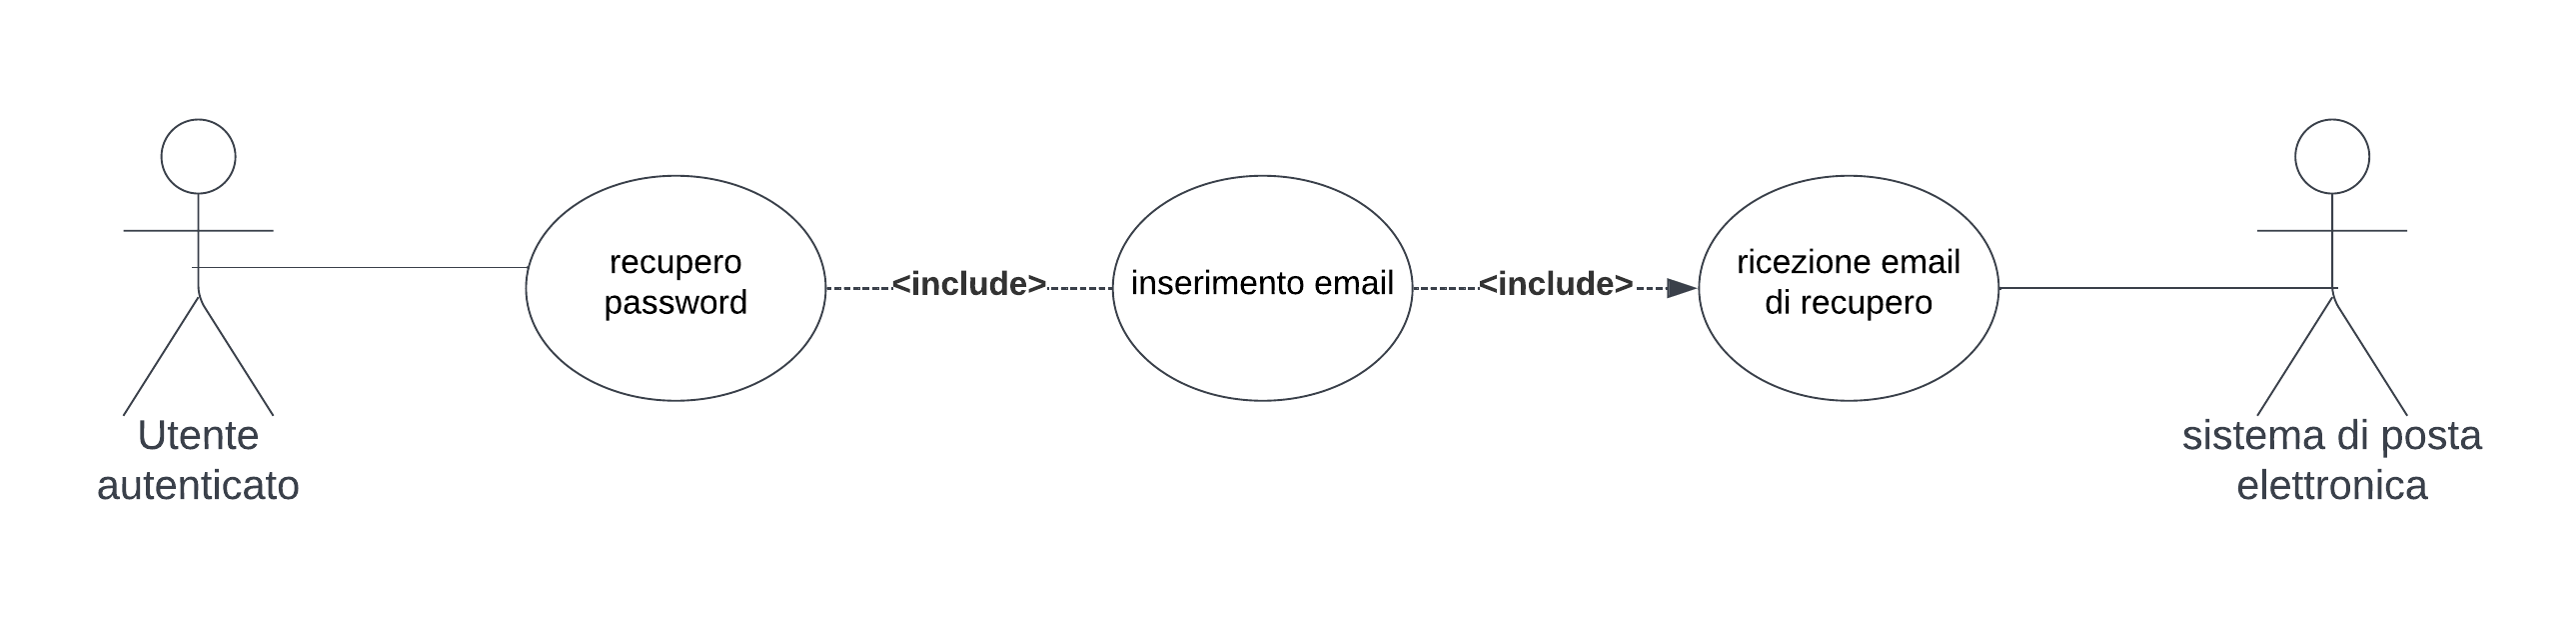
\includegraphics[width=0.7\textwidth]{img/Diagrammi/UseCases/RecuperoPassword.png}
    \end{center}


    \textbf{Diagramma:}
    \begin{center}
        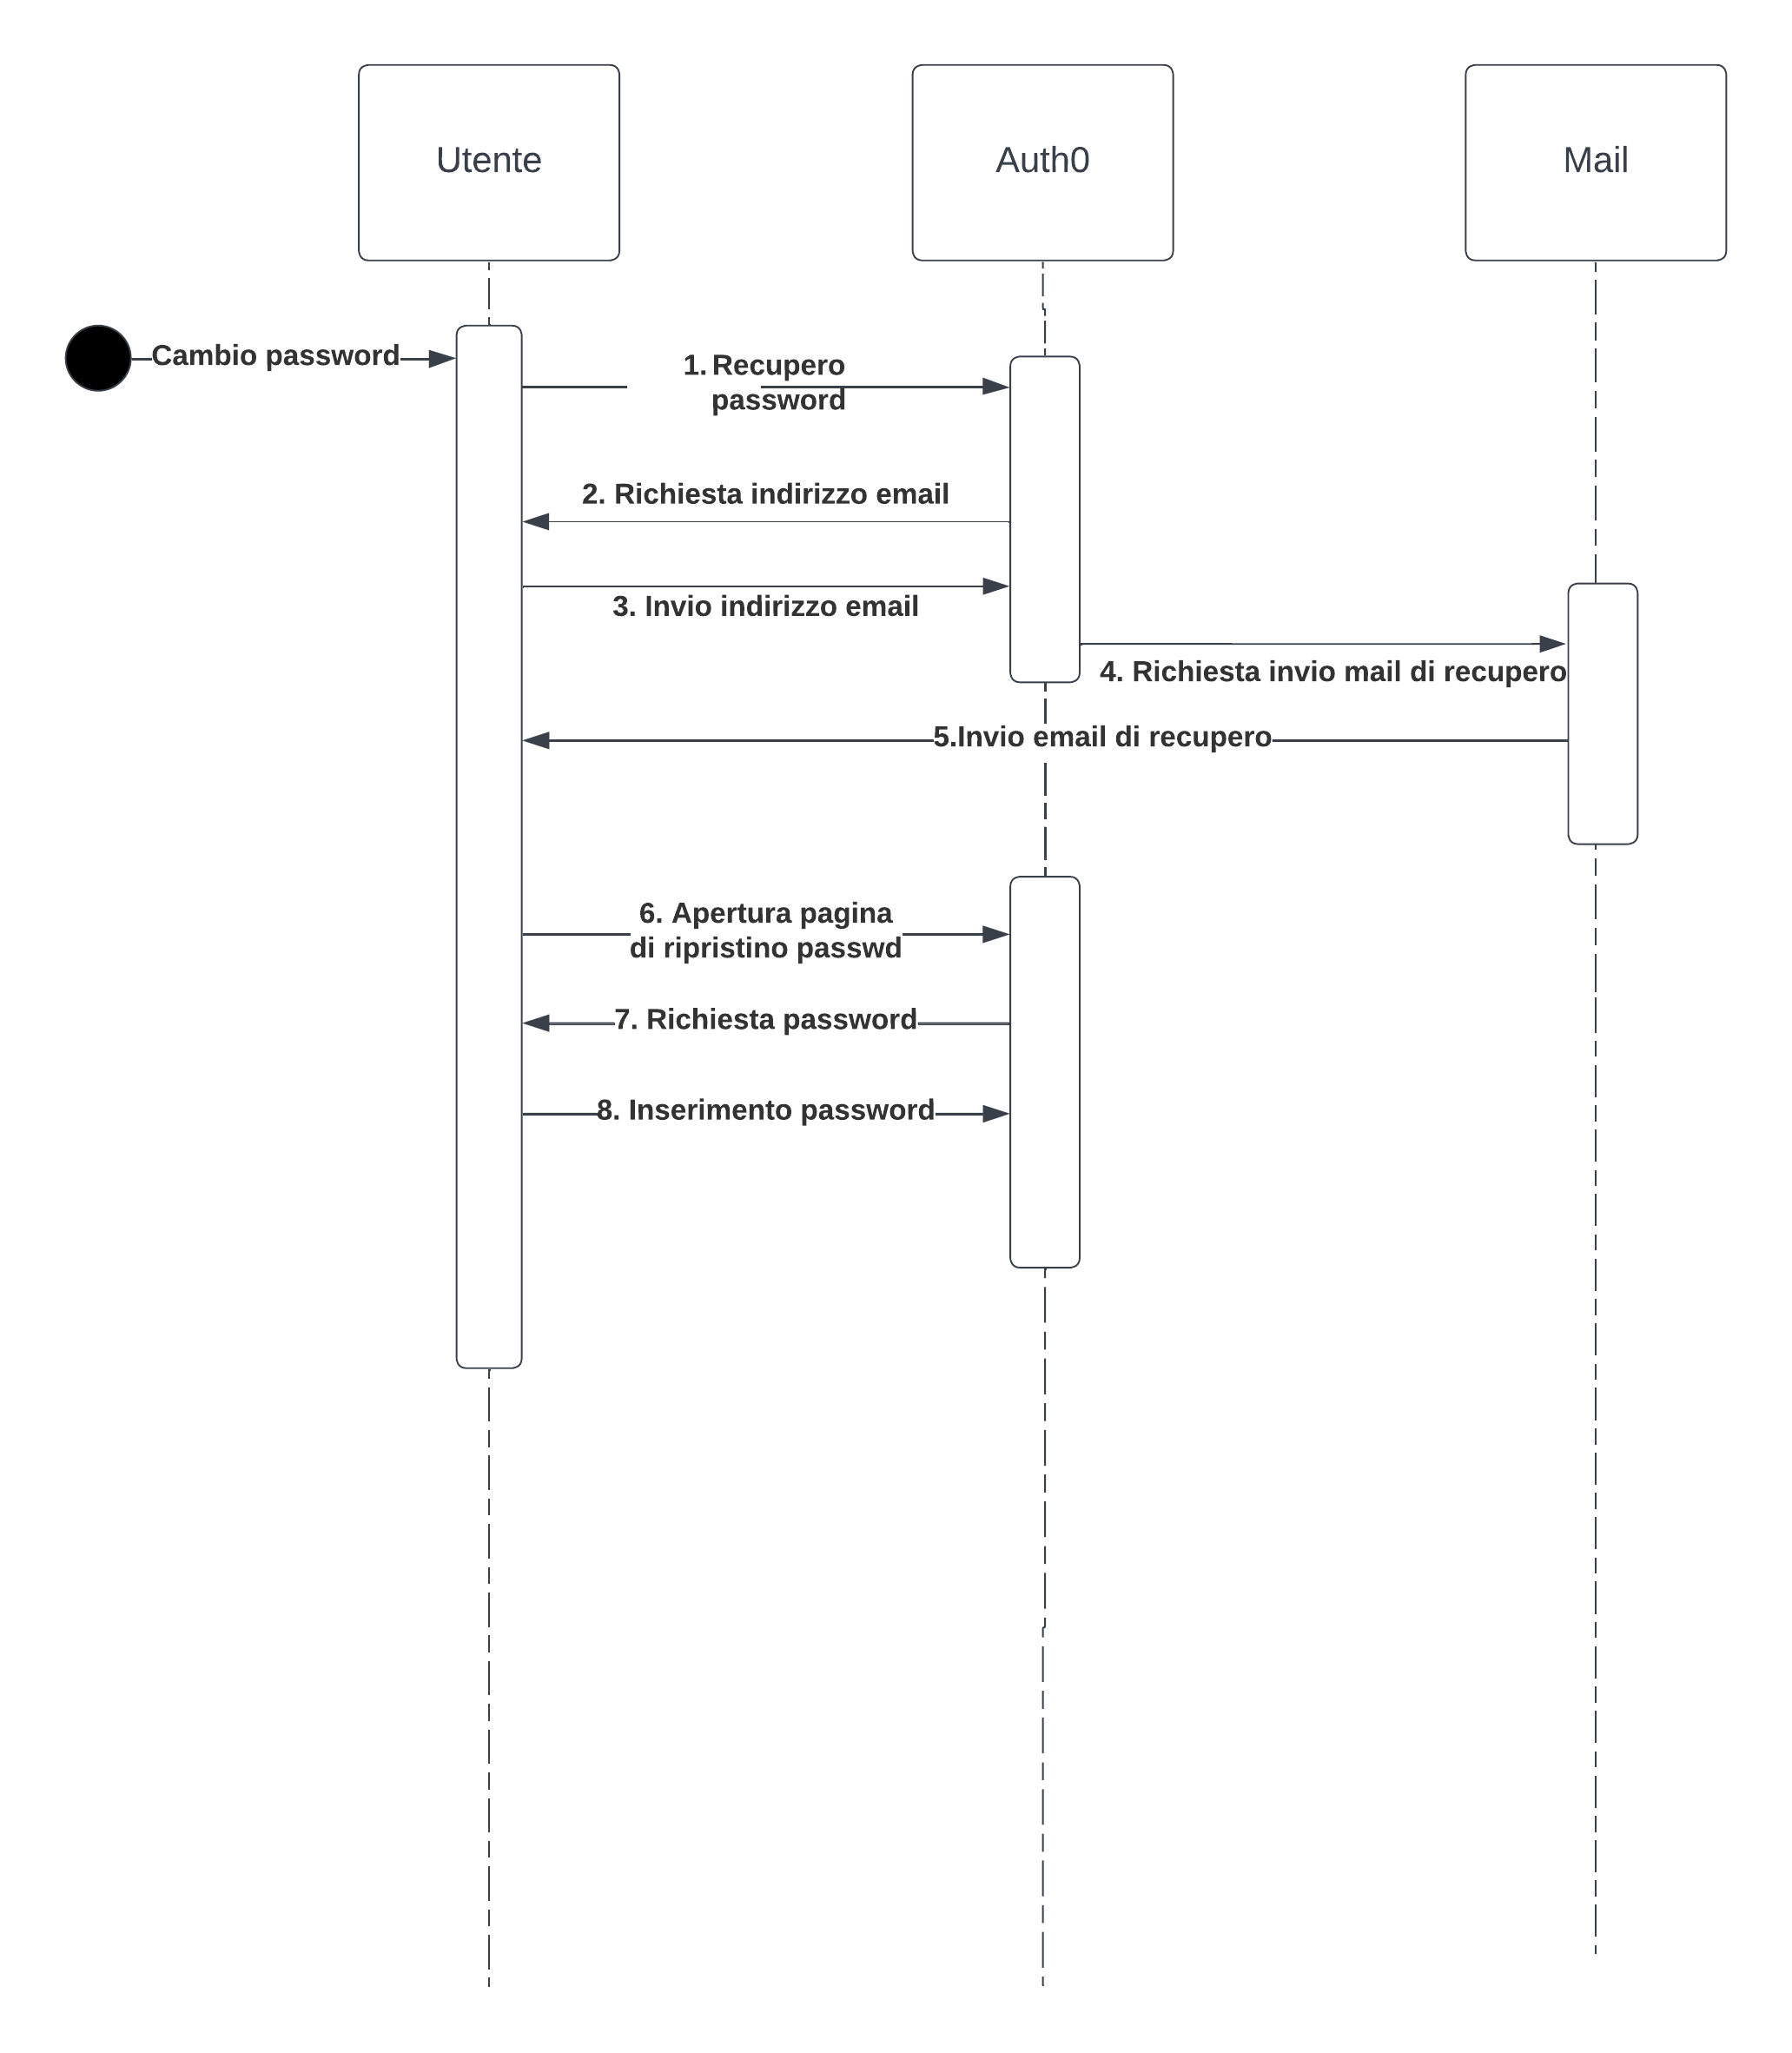
\includegraphics[width=0.7\textwidth]{img/Diagrammi/DS/DS_RecuperoPassword.png}
    \end{center}

\end{listaPersonale}